\chapter{Methods}
\label{chap:3}
In this chapter, the \glspl{NFCSim}, \Cyclus and DYMOND, will 
be described. 
A new capability in \Cyclus to ease setting up 
of transition scenarios that was developed for this work 
will also be described. 

\section{\Cyclus}
\Cyclus is an agent-based nuclear fuel cycle simulation framework 
\cite{huff_fundamental_2016}. 
In \Cyclus, each entity (i.e. Region, Institution, or Facility) in 
the fuel cycle is an agent. 
Region agents represent geographical or political areas that institution
and facility agents can be grouped into. 
Institution agents control the 
deployment and decommission of facility agents 
and represents legal operating organizations such as a 
utility, government, etc. \cite{huff_fundamental_2016}. 
Facility agents represent nuclear fuel cycle facilities. 
\Cycamore \cite{carlsen_cycamore_2014}
provides facility agents to represent process physics of various 
components in the nuclear fuel cycle (e.g. mine, fuel enrichment 
facility, reactor). 
The \Cycamore reactor model uses externally-calculated 
recipes for fresh and spent fuel compositions. 
The mass flows and inventories are recorded at an agent-level
and individual isotopes are tracked. 

% Describe the agent-based model and flexibility
Two of \Cyclus' main design objectives are user customization and 
extensibility. 
These objectives are achieved through \Cyclus' modularity, 
open architecture, and agent interchangeability. 
The modularity and open architecture provides users with a 
platform to develop custom facilities with their chosen fidelity 
and capabilities. 
Agent interchangeability facilitates setting up of custom fuel 
cycles and direct comparisons of alternative modeling methodologies 
and facility concepts \cite{huff_fundamental_2016}. 

In 2016, there was a push to understand and evaluate the 
transition from the initial EG01 state to promising future 
end-states \cite{feng_standardized_2016}.
Previously in \Cyclus, reactor facilities are automatically 
deployed to meet a user-defined power demand. 
However, it is up to the user to define a deployment scheme of 
supporting facilities to ensure that there is no gap in the supply 
chain that results in idle reactor capacity. 
To avoid this issue, users 
have to set infinite capacities for the support facilities, 
but this is an inaccurate representation of reality. 
Another option is to manually calculate a suitable deployment 
schedule. 
It is straightforward to manually determine a deployment scheme 
for a once-through fuel cycle, however, it is difficult to effectively 
implement for complex closed fuel cycle scenarios.  
Therefore, to successfully conduct analysis of the time-dependent 
closed fuel cycle transition
analyses, it is necessary to develop \gls{NFCSim} tools to  
automate setting up of transition scenarios. 
Therefore, Demand-Driven Cycamore Archetypes project
(NEUP-FY16-10512) was initiated to develop demand-driven deployment 
capabilities in \Cyclus.
This capability is added as a \Cyclus Institution
agent that deploys facilities to meet the front-end and back-end 
fuel cycle demands based on a user-defined commodity demand. 
This demand-driven deployment capability is called 
\deploy. 

\subsection{\deploy's Capabilities}
\label{sec:d3ploy}
In a \Cyclus simulation, at every timestep, \deploy 
predicts supply and demand of each commodity for the next time 
step. 
If there is an undersupply of any commodity based 
on the predicted values, \deploy deploys facilities to meet 
the predicted demand.  
Figure \ref{fig:flow} shows the logic flow of \deploy 
at every timestep. 

\begin{figure}[]
    \centering
    \caption{\deploy logic flow at every timestep in \Cyclus \cite{chee_demonstration_2019}.}
    \label{fig:flow}
    \begin{tikzpicture}[node distance=2.5cm]
        \tikzstyle{every node}=[font=\large]
        \node (Start) [bblock] {\textbf{Start of timestep ($t$).}};
        \node (Predict) [bblock, below of=Start] {\textbf{Calculate \\ $D_p(t+1)$ and $S_p(t+1)$ for a commodity}};
        \node (IsThere) [oblock, below of=Predict]{\textbf{$U(t+1) = S_p(t+1)-D_p(t+1)$}};
        \node (Deploy) [sbblock, below of=IsThere, xshift = -3.5cm]{\textbf{Deployment \\ of facility}};
        \node (NoDeploy) [sbblock, right of=Deploy, xshift = 3.5cm]{\textbf{No Deployment} };
        \node (All) [oblock, below of=Deploy, xshift = 3.5cm] {\textbf{Is this done for all commodities?}};
        \node (End) [bblock, below of=All] {\textbf{Proceed to next timestep.}};
        
        \draw [arrow] (Start) -- (Predict); 
        \draw [arrow] (Predict) -- (IsThere);
        \draw [arrow] (IsThere) -- node[anchor=east] {$U(t+1) <$ buffer} (Deploy);
        \draw [arrow] (IsThere) -- node[anchor=west] {$U(t+1) \geq$ buffer} (NoDeploy);
        \draw [arrow] (Deploy) -- (All);
        \draw [arrow] (NoDeploy) -- (All);
        \draw [arrow] (All) -- node[anchor=west] {yes} (End);
        \draw [arrow] (All) -- ([shift={(-3.9cm,0.7cm)}]All.south west)-- node[anchor=east] {no} ([shift={(-3.9cm,-0.85cm)}]Predict.north west)--(Predict);
        \draw [arrow] (End) |-([shift={(3cm,-0.5cm)}]End.south east)-- ([shift={(3cm,0.5cm)}]Start.north east)-|(Start);
    \end{tikzpicture}
\end{figure}

\deploy's overall objective is to ensure that there is no 
undersupply of power. 
The sub-objectives are : (1) to minimize the number of time 
steps of undersupply or under capacity of any 
commodity, (2): to minimize excessive oversupply of all commodities.
This is a reflection of reality in which it is important to 
never have an undersupply of power on the grid by ensuring power 
plants are never undersupplied of fuel, while not 
having excessive over supply resulting in a burden to store unused 
supplies. 
One of the key issues that \gls{NFCSim}s face is that despite
sufficient installed reactor capacity to meet the power 
demand, there is insufficient supply of fabricated/reprocessed 
fuel at certain timesteps, resulting in idle capacity.  

\subsubsection{\textbf{Structure}}
%Description of front end and back end of fuel cycle 
%Demand Driven vs. Supply Driven 
In \deploy, two different institutions were implemented for 
front-end and back-end fuel cycle facilities: 
\texttt{DemandDrivenDeploymentInst} and 
\texttt{SupplyDriven} 
\noindent
\texttt{DeploymentInst} respectively. 
This distinction was made because front-end facilities 
are deployed to meet demand for the commodity they produce. 
Whereas, back-end facility are deployed to meet supply for the 
commodity they provide capacity for. 
For example, for front end facilities, a reactor facility 
demands fuel and \texttt{DemandDrivenDeploymentInst} 
triggers deployment of fuel fabrication facilities to create 
supply meeting demand for fuel to prevent undersupply. 
For back end facilities, the reactor generates spent fuel and 
\texttt{SupplyDrivenDeploymentInst} triggers deployment of 
waste storage facilities to create capacity meeting the supply 
of spent fuel to prevent under capacity. 

\subsubsection{\textbf{Input Variables}}
Table \ref{tab:inputs} lists and gives examples of the input 
variables \deploy accepts. 
Essentially, the user must define the facilities controlled by 
\deploy, their respective capacities, the driving commodity, 
its demand equation, deployment driving method, and prediction method 
for supply and demand. 
The user also has the optional option to define supply/capacity buffers 
for each commodity, facility preferences, and facility constraints. 
In-depth descriptions of the deployment driving method, prediction 
methods, preferences, and buffers are provided in the subsequent sections. 

\begin{table}[]
    \centering
	\resizebox{0.7\textwidth}{!}{%
	\begin{tabular}{|l|l|p{7cm}|}
	\hline
											  & \textbf{Input Parameter}                                                           & \textbf{Examples}                                                                                                          \\ \hline
	\multirow{5}{*}{\textbf{Required}} & Demand driving commodity                                                           & Power, Fuel, Plutonium, etc.                                                                                                                      \\ \cline{2-3} 
											  & Demand equation                                                                    & P(t) = 10000, sin(t), 10000*t                                                                                                                 \\ \cline{2-3} 
											  & Facilities it controls                                                             & Fuel Fab, LWR reactor, SFR reactor, Waste repository, etc.                                                                                                      \\ \cline{2-3} 
											  & Capacities of the facilities                                                       & 3000 kg, 1000 MW, 50000 kg                                                                                                     \\ \cline{2-3} 
											  & Prediction method                                                                  & \begin{tabular}[c]{@{}l@{}}Power: fast fourier transform\\ Fuel: moving average\\ Spent fuel: moving average\end{tabular} \\ \cline{2-3} 
											  & Deployment driven by & Installed Capacity/Supply                                                                                                                    \\ \hline
	\multirow{4}{*}{\textbf{Optional}} & Supply/Capacity Buffer type                                                                        & Absolute                                                                                                                  \\ \cline{2-3} 
											  & Supply/Capacity Buffer size                                                                        & \begin{tabular}[c]{@{}l@{}}Power: 3000 MW\\ Fuel: 0 kg \\ Spent fuel: 0 kg\end{tabular}                                   \\ \cline{2-3} 
											  & Facility preferences                                                               & \begin{tabular}[c]{@{}l@{}}LWR reactor = 100-t\\ SFR reactor = t-100 \end{tabular}          \\ \cline{2-3} 
											  & Facility constraint                                                              & SFR reactor constraint = 5000kg of Pu            \\ \hline	
			
											\end{tabular}%
	}
	\caption{\deploy's required and optional input parameters with examples.}
	\label{tab:inputs}
    \end{table}

    \subsubsection{\textbf{Deployment Driving Method}}
    The user has the choice of deploying facilities based on the difference 
    between predicted supply and demand, or predicted demand and 
    installed capacity. 
    There are two advantages of using installed capacity over predicted 
    supply. 
    First, to prevent over deployment of facilities that have an
    intermittent supply. 
    For example, reactor facilities have a periodic refueling time. 
    A user might not want \deploy to deploy more reactor facilities 
    to make up for the lack of power supply caused by the gap in 
    supply during refueling. 
    Second, to prevent infinite deployment of a facility that uses 
    a commodity that is no longer available in the simulation. 
    For example, in a transition scenario from \gls{LWR}s to \gls{SFR}s, 
    the reprocessing plant that fabricates \gls{SFR} fuel might demand 
    Pu after the inventory accumulated by \gls{LWR}s is used up 
    and there are no more \gls{LWR} facilities to generate Pu. 
    This will result in \deploy deploying infinite reprocessing 
    facilities to generate \gls{SFR} fuel despite the lack of input Pu 
    to generate it. 
    This can be avoided by using \deploy's facility constraint capability 
    to constrain \gls{SFR} deployment until a sizable inventory of Pu 
    is accumulated in the simulation. 
    
    \subsubsection{\textbf{Supply/Capacity Buffer}}
    In \texttt{DemandDrivenDeploymentInst}, the user has the option 
    to provide a supply buffer for each commodity so that 
    \deploy will deploy facilities to meet predicted demand and the
    additional buffer value. 
    In \texttt{SupplyDrivenDeploymentInst}, the user has the option 
    to provide a capacity buffer to specific commodities so that 
    \deploy will deploy facilities to meet predicted supply and the
    additional buffer.
    For example, the user could set the power commodity's supply buffer 
    to be 2000 MW. 
    If predicted demand is 10000 MW, \deploy will deploy reactor 
    facilities to meet the predicted demand and supply buffer, resulting 
    in a power supply of 12000 MW.  
    The buffer can be defined as a percentage (equation \ref{eq:perc}) 
    or absolute value (equation \ref{eq:abs}). 
    
    \begin{equation}
        \label{eq:perc}
        S_{pwb} = S_{p}*(1+d)
    \end{equation}
    \begin{equation}
        \label{eq:abs}
        S_{pwb} = S_{p}+a
    \end{equation}
    where $S_{pwb}$ is predicted supply/capacity with buffer, 
    $S_p$ is the predicted supply/capacity without buffer, 
    $d$ is the percentage value in decimal form, 
    and $a$ is the absolute value of the buffer. 
    
    Using a combination of this buffer capability with the 
    installed capacity deployment driving method in a transition 
    scenario simulation is effective in minimizing undersupply of a 
    commodity without having excessive over supply. 
    This is demonstrated in section \ref{sec:demo}. 
    
    \subsubsection{\textbf{Preferences}}
    % Need to explain the order of preferences for deployment 
    % Constraint, pref, minimize number of facilities and minimize 
    % over supply 
    The user has the option to provide each facility with
    a time dependent preference equation that governs preference for 
    that facility compared to other facilities that provide the same 
    commodity. 
    In the example for facility preferences in table \ref{tab:inputs}, 
    the \gls{LWR} reactor has a preference of $100-t$ and the 
    \gls{SFR} reactor has a preference of $t-100$. 
    Thus, the \gls{LWR} is preferred before time step 100 and \gls{SFR}
    is preferred after. 
    
    The user also has the option to provide each facility with a 
    commodity constraint. 
    In the example for facility constraint in table \ref{tab:inputs}, 
    the \gls{SFR} has a commodity constraint of 5000kg of Pu. 
    This constrains \gls{SFR} deployment by the size of the Pu inventory 
    in the simulation. 
    Once, the 5000kg Pu inventory is first met, \gls{SFR} reactors can 
    henceforth be deployed. 
    
    One of the key issues faced in transition scenarios is the lack 
    of Pu in a scenario that results in idle advanced reactor capacity. 
    Therefore, the facility preferences and constraint capabilities 
    are useful and necessary for modeling transition scenarios. 
    An ideal transition year is selected using the facility 
    preferences, however the transition will only begin when there 
    is sufficient Pu inventory (set by facility constraint) 
    to avoid Pu shortages. 
    
    Therefore, when \deploy predicts an undersupply of a commodity, 
    it deploys available facilities to meet the predicted demand. 
    It will deploy the facility with the highest preference first, 
    unless it does not meet it's constrained criteria, then it will 
    deploy the second most, and so on. 
    If the facilities do not have preferences or constraints, \deploy 
    will deploy the available facilities to minimize the number of 
    deployed facilities while minimizing oversupply of the commodity.

\subsubsection{\textbf{Prediction Methods}}

\subsection{\deploy Demonstration}
\label{sec:demo}

This section will demonstrate \deploy's capability 
to effectively conduct simple transition scenario analysis
for constant, linearly increasing, and 
sinusoidal power demand simulations.
These simulations are basic transition scenarios that only include 
three types of facilities: \texttt{source}, \texttt{reactor}, and 
\texttt{sink}. 
All simulations have ten initial \texttt{reactor} facilities 
(\texttt{reactor1} to \texttt{reactor10}). 
These reactors have staggered cycle lengths and lifetimes to prevent 
simultaneous refueling and set up gradual decommissioning. 
\deploy is set up to deploy \texttt{new reactor} facilities
to meet the loss of power supply introduced from the decommissioning 
of the initial \texttt{reactor} facilities. 
The \deploy input parameters for each simulation is shown in Table 
\ref{tab:demonstrations}. 
Figure \ref{fig:powerplots} shows the user-defined power demand curves 
that \deploy needs to deploy facilities meet for each simulation.

\begin{table}[]
    \resizebox{\textwidth}{!}{%
    \begin{tabular}{|l|l|c|l|l|}
    \hline
    \multirow{2}{*}{}                         & \multicolumn{1}{c|}{\multirow{2}{*}{\textbf{Input Parameter}}} & \multicolumn{3}{c|}{\textbf{Simulation Description}}                                                                                                                                                                                                                                                       \\ \cline{3-5} 
                                              & \multicolumn{1}{c|}{}                                          & \multicolumn{1}{l|}{\textbf{Constant Power}}                                                                 & \textbf{\begin{tabular}[c]{@{}l@{}}Linearly Increasing \\ Power\end{tabular}}                  & \textbf{Sinusoidal Power}                                                                  \\ \hline
    \multirow{5}{*}{\textbf{Required Inputs}} & Demand driving commodity                                       & \multicolumn{3}{c|}{Power}                                                                                                                                                                                                                                                                                 \\ \cline{2-5} 
                                              & Demand equation                                                & \multicolumn{1}{l|}{10000 MW}                                                                                & \begin{tabular}[c]{@{}l@{}}t\textless 40: 10000 MW\\ t\textgreater{}=40: 250*t MW\end{tabular} & 1000*$\sin(\pi*t/3)$+10000                                                                 \\ \cline{2-5} 
                                              & Facilities it controls                                         & \multicolumn{3}{c|}{Source, reactor, sink}                                                                                                                                                                                                                                                                 \\ \cline{2-5} 
                                              & Prediction method                                              & \multicolumn{1}{l|}{\begin{tabular}[c]{@{}l@{}}Power: FFT\\ Fuel: MA\\ Spent fuel: MA\end{tabular}}          & \begin{tabular}[c]{@{}l@{}}Power: FFT\\ Fuel: MA\\ Spent fuel: FFT\end{tabular}                & \begin{tabular}[c]{@{}l@{}}Power: HW\\ Fuel: MA\\ Spent fuel: FFT\end{tabular}             \\ \cline{2-5} 
                                              & Deployment Driving Method                                      & \multicolumn{3}{c|}{Installed Capacity}                                                                                                                                                                                                                                                                    \\ \hline
    \multirow{2}{*}{\textbf{Optional Inputs}} & Buffer type                                                    & \multicolumn{3}{c|}{Absolute}                                                                                                                                                                                                                                                                              \\ \cline{2-5} 
                                              & Buffer size                                                    & \multicolumn{1}{l|}{\begin{tabular}[c]{@{}l@{}}Power: 3000 MW\\ Fuel: 0 kg \\ Spent fuel: 0 kg\end{tabular}} & \begin{tabular}[c]{@{}l@{}}Power: 2000 MW\\ Fuel: 1000 kg \\ Spent fuel: 0 kg\end{tabular}     & \begin{tabular}[c]{@{}l@{}}Power: 2000 MW\\ Fuel: 1000 kg \\ Spent fuel: 0 kg\end{tabular} \\ \hline
    \end{tabular}%
    }
    \caption{\deploy's input parameters for the basic transition scenarios.}
    \label{tab:demonstrations}
    \end{table}

    \begin{figure}[]
        \begin{center}
            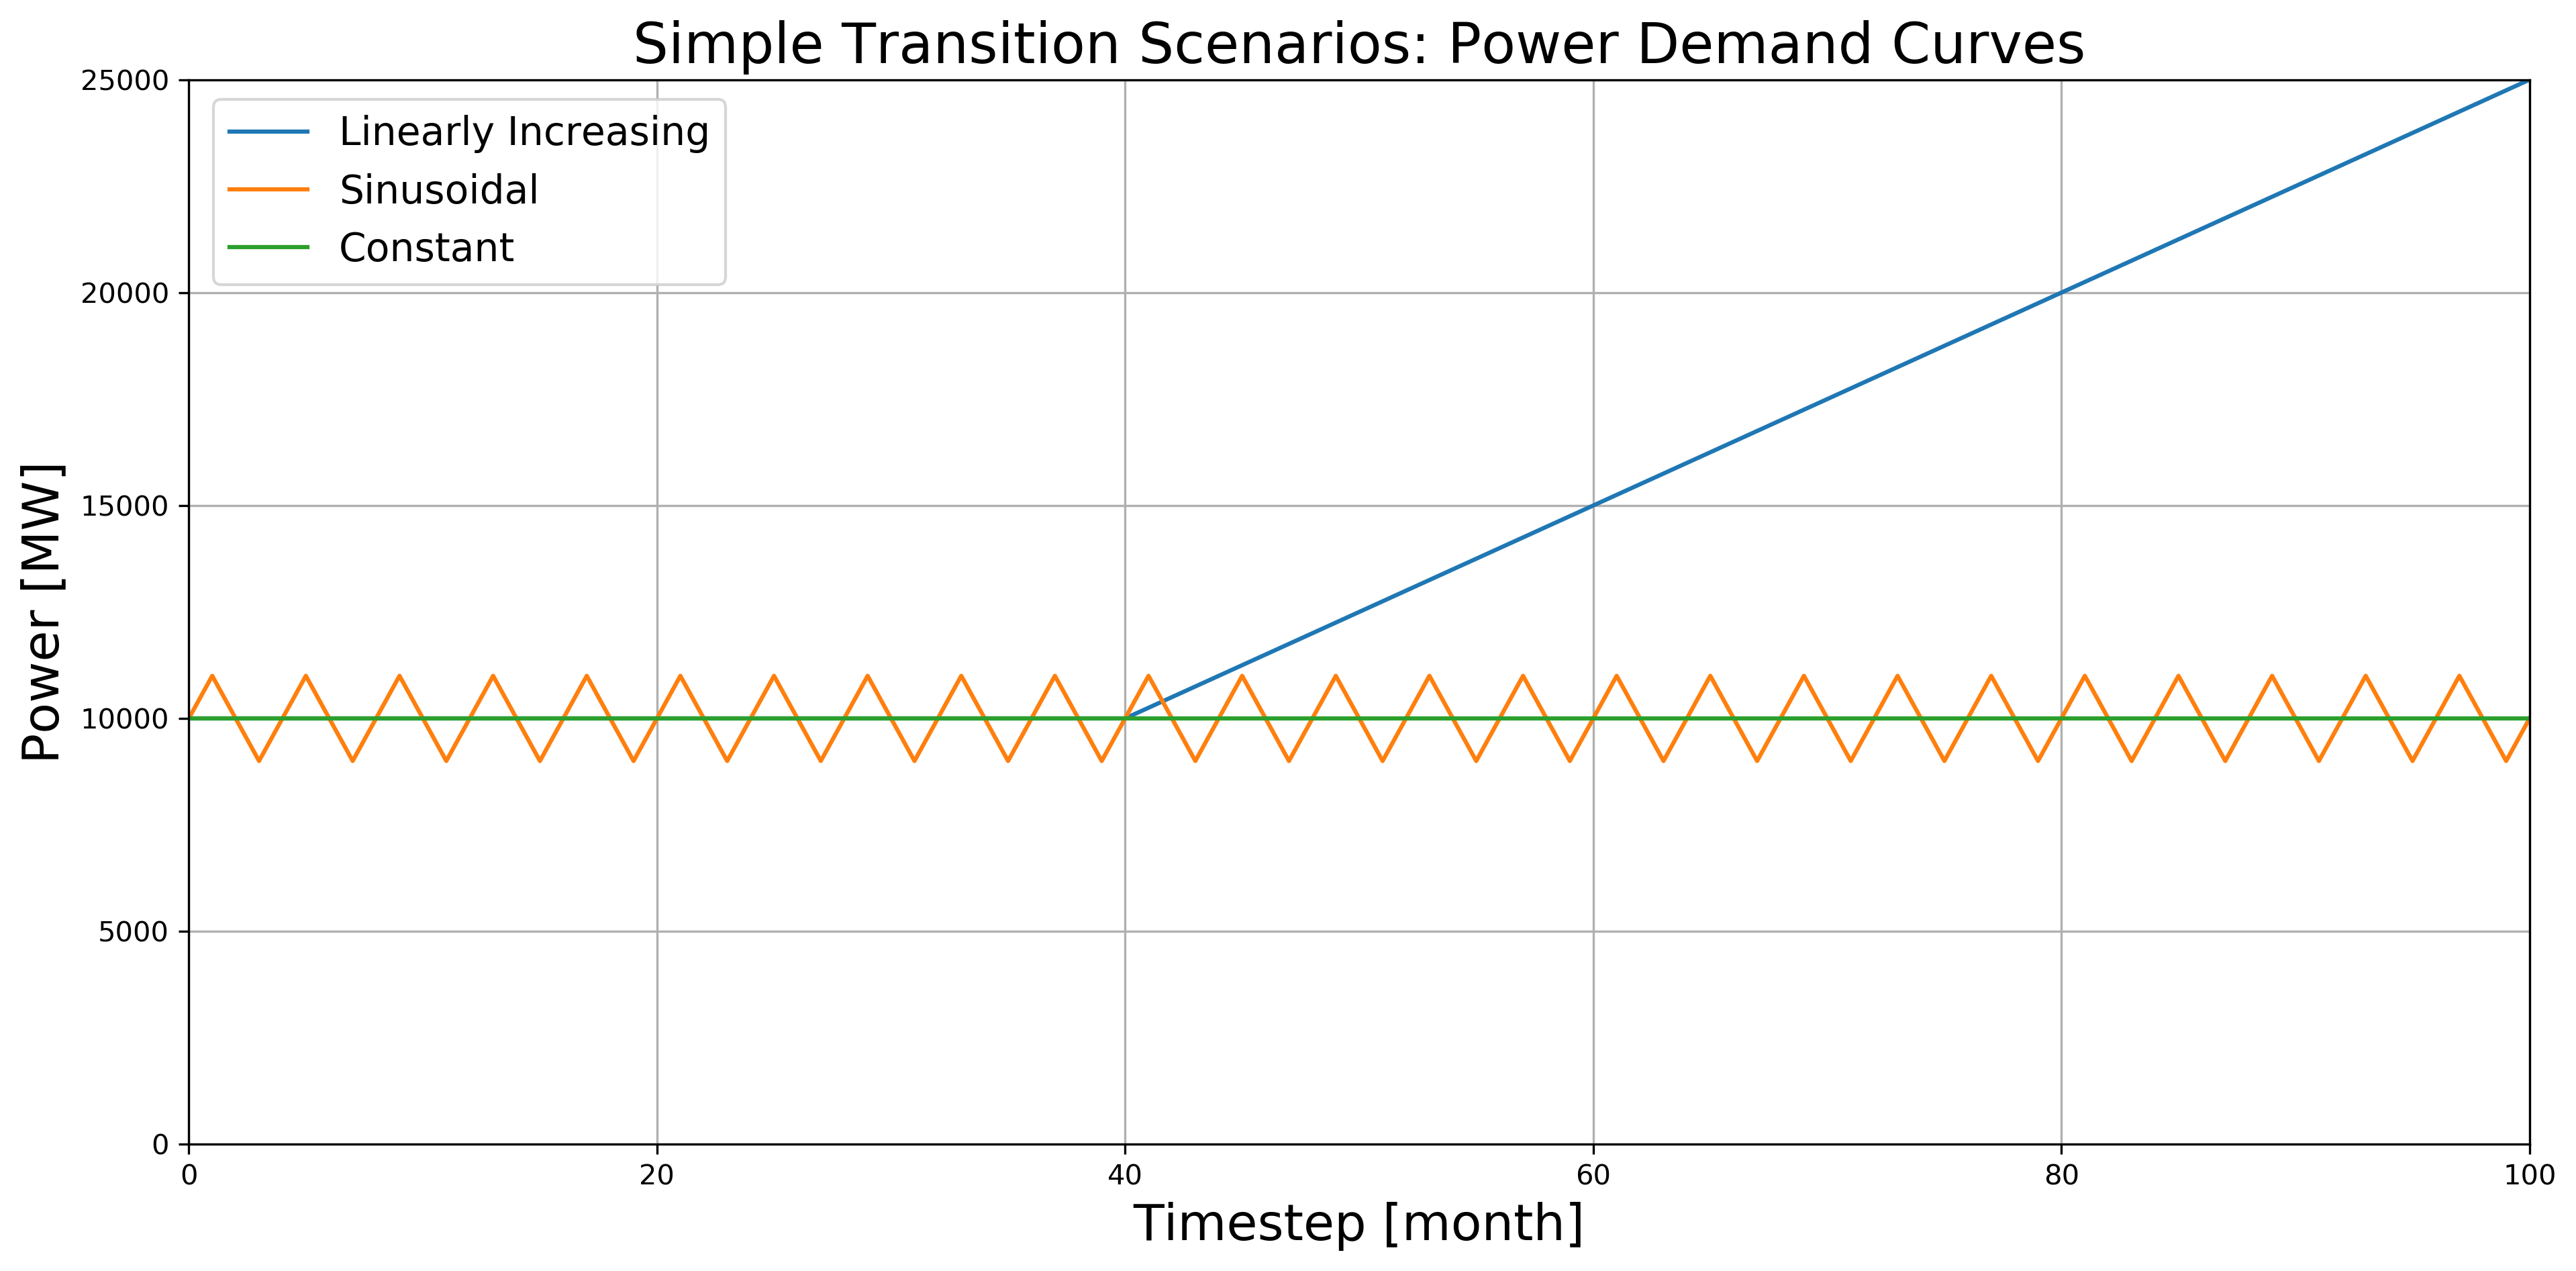
\includegraphics[scale=0.37]{./figures/powerplots.png}
        \end{center}
            \caption{Power demand curves for basic transition scenarios.}
        \label{fig:powerplots}
    \end{figure}

\subsubsection{\textbf{Basic Transition Scenario Simulation: Constant Demand}}
Figures \ref{fig:constanttransition-power}, \ref{fig:constanttransition-fuel}
and \ref{fig:constanttransition-spentfuel} demonstrate \deploy's capability 
to deploy reactor and supporting facilities to meet the user 
determined constant power demand and subsequently demanded 
secondary commodities with minimal undersupply. 
Table \ref{tab:transition-scenario-results} shows the number of 
undersupplied timesteps. 
Figure \ref{fig:constanttransition-power} demonstrates that
the main objective of \deploy (section \ref{sec:d3ploy}) 
was met since there are no timesteps
in which the supply of power falls under demand.
By using a combination of the fast fourier transform method for 
predicting demand and setting the supply buffer to 3000MW 
(the capacity of 3 reactors), the user minimizes the number of 
undersupplied timesteps for every commodity.

In figure \ref{fig:constanttransition-fuel},
a facility with a large fuel throughput is initially
deployed to meet the large initial fuel demand for the starting
up of ten reactors. 
\deploy is prevented from deploying many supporting
facilities that end up being redundant at the later parts of 
the simulation, by having an initial facility with a large throughput
exist for the first few timesteps in the simulation.
This is a reflection of reality in which reactor manufacturers will 
accumulate an appropriate amount of fuel inventory before starting 
up reactors. 
There is one timestep where there is an undersupply after the 
decommissioning of the large initial facility.  
This is unavoidable since the prediction methods in \deploy are 
unable to predict this sudden drop in demand. 

    \begin{figure}[]
        \centering
        \begin{subfigure}[t]{\textwidth}
        \centering
            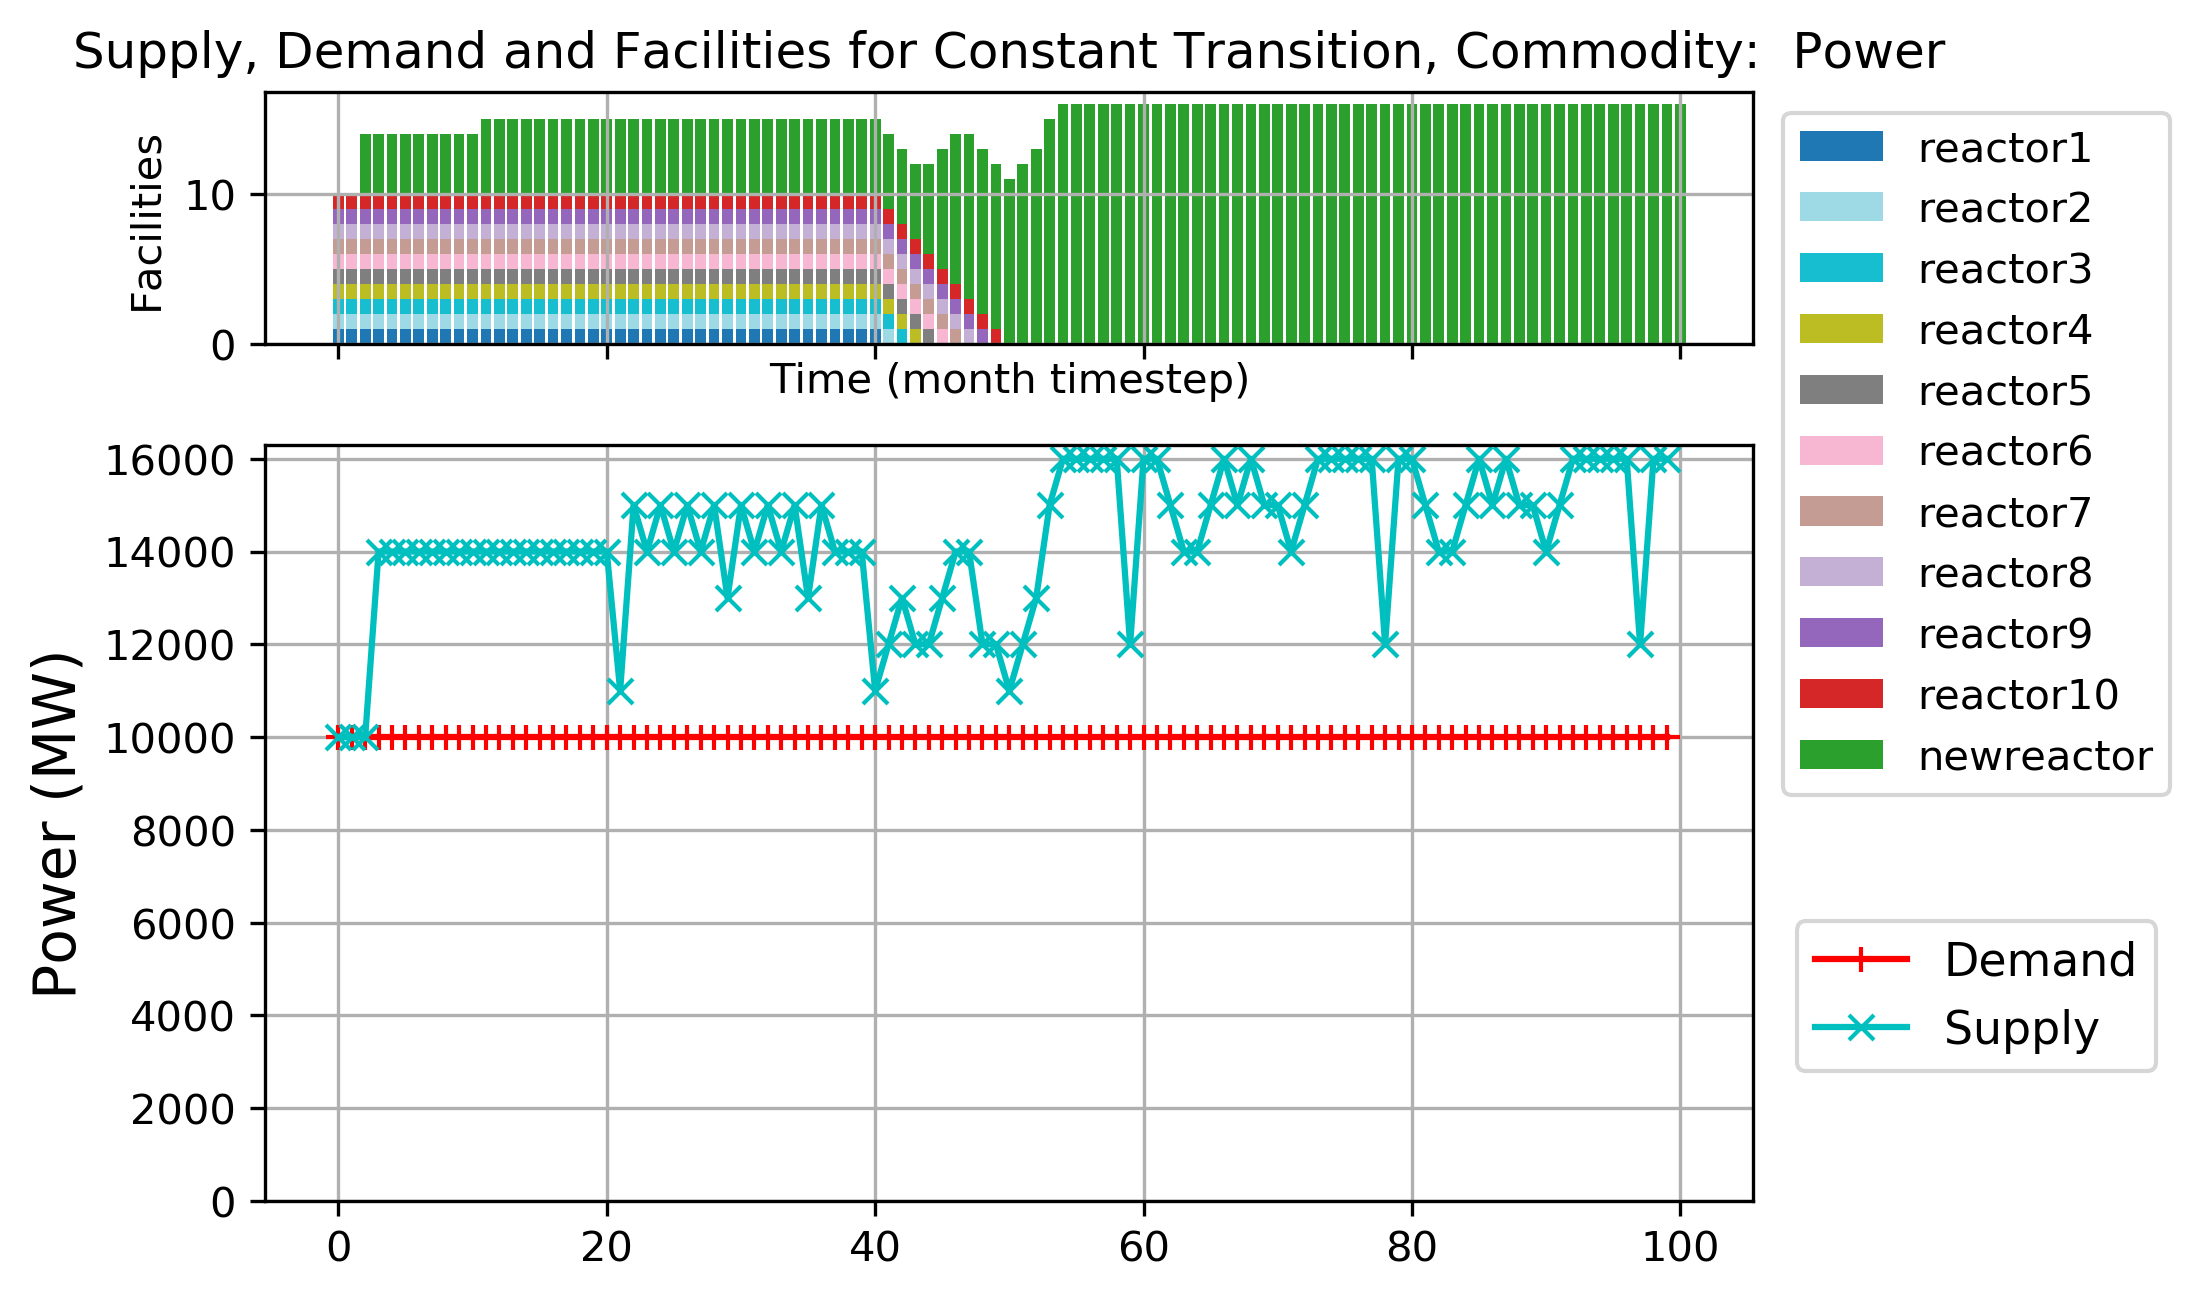
\includegraphics[width=0.7\linewidth]{figures/constanttransition-power.png} 
            \caption{The power demand is a user-defined equation and power is supplied by the reactors.}
            \label{fig:constanttransition-power}
        \end{subfigure}
        \begin{subfigure}[t]{0.6\textwidth}
            \centering
            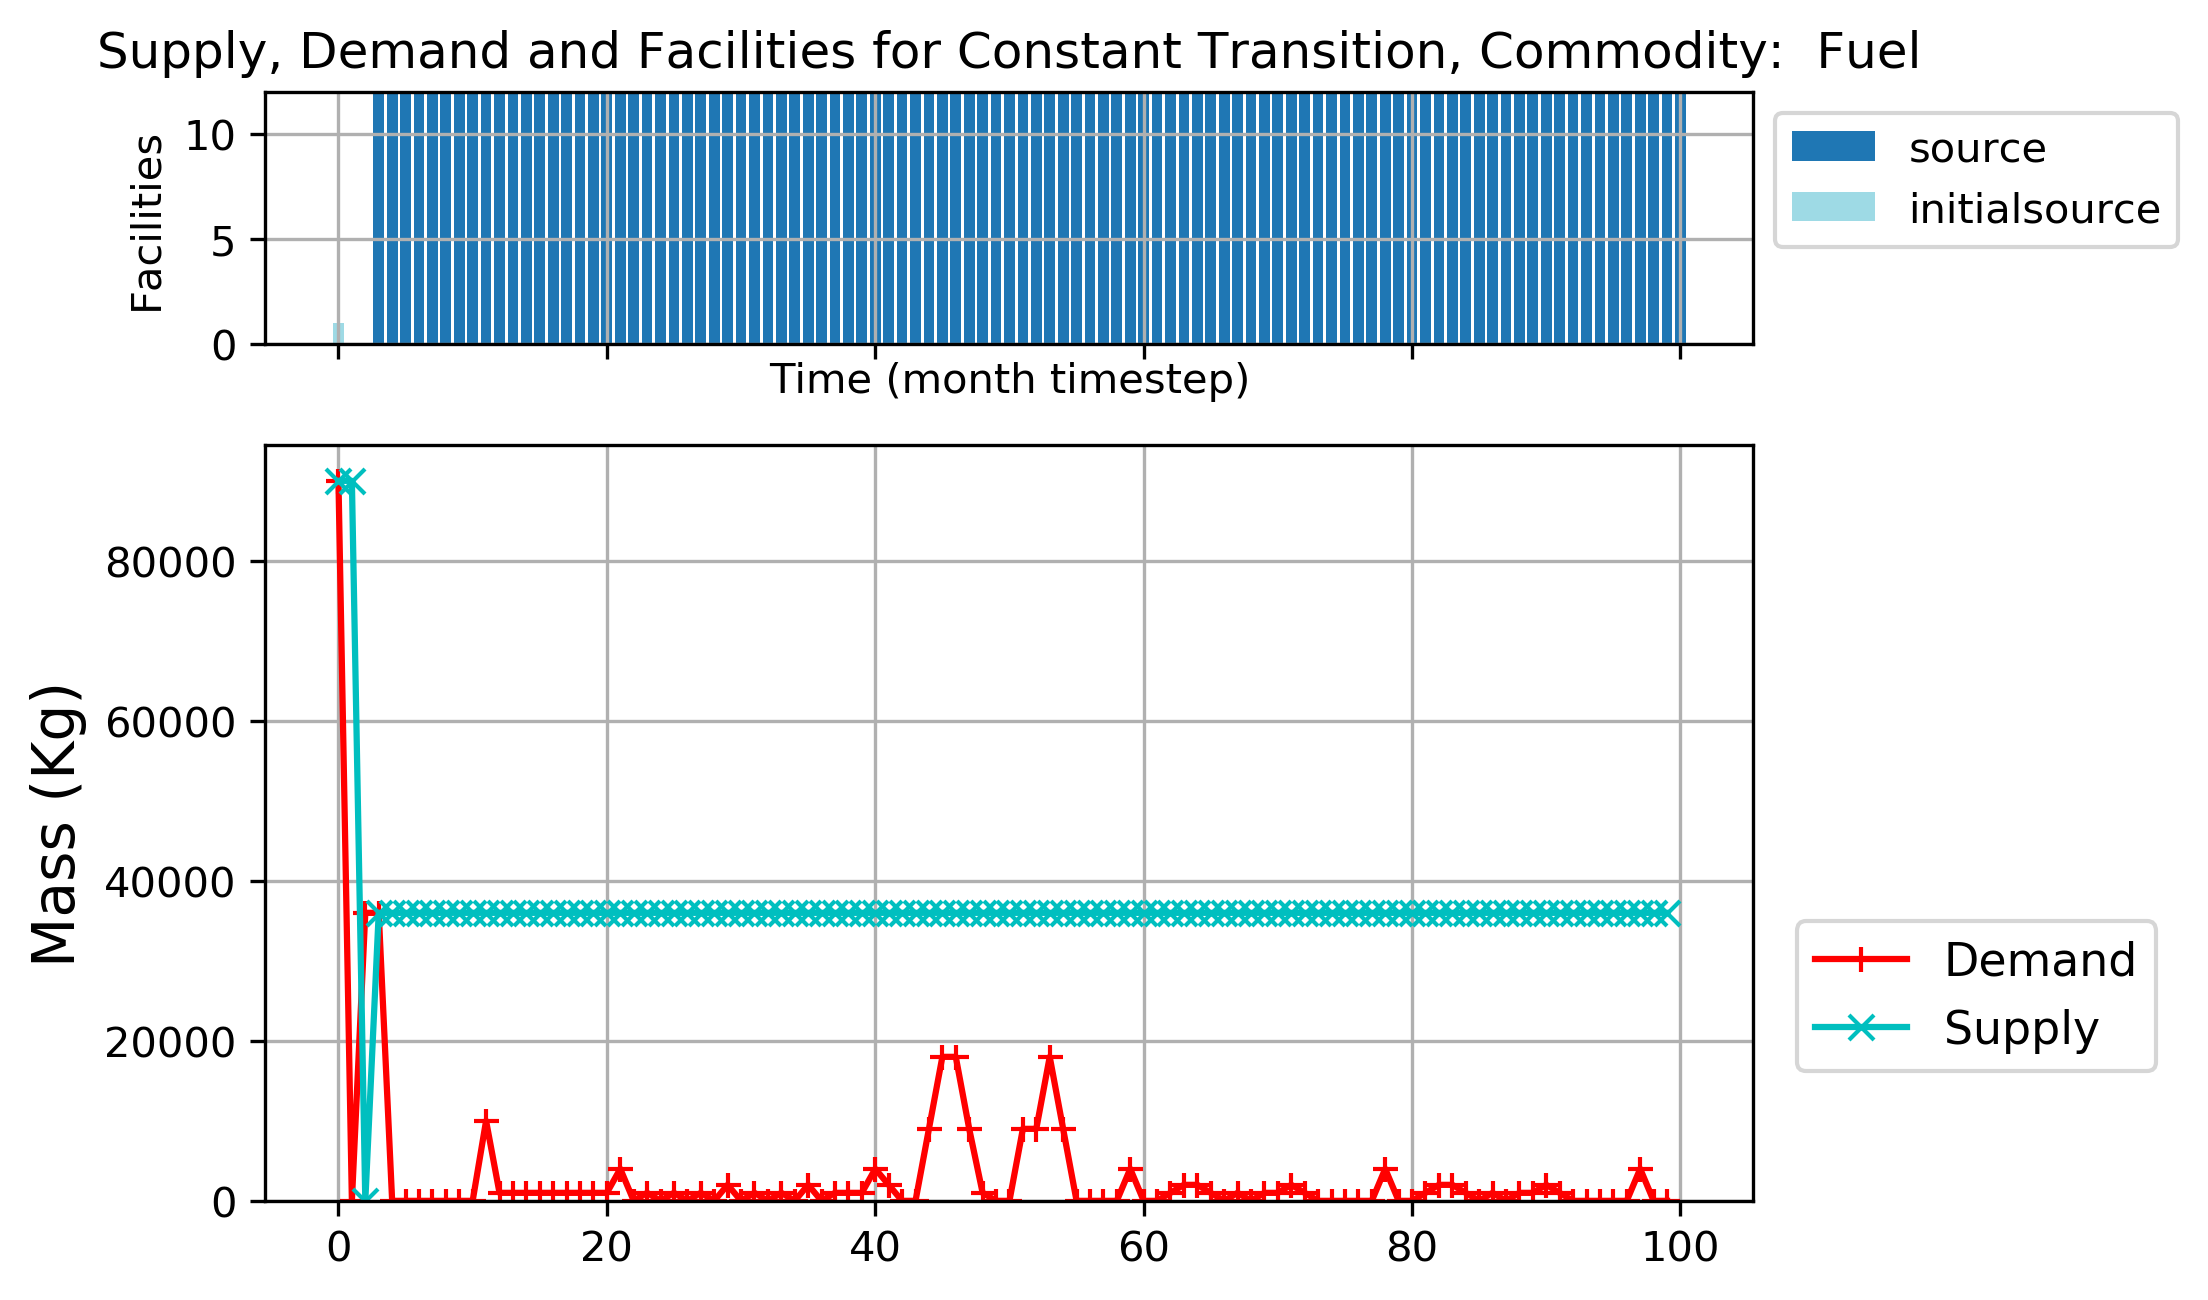
\includegraphics[width=\linewidth]{figures/constanttransition-fuel.png} 
            \caption{Fuel is demanded by reactors and supplied by source facilities.}
            \label{fig:constanttransition-fuel}
        \end{subfigure}
        \begin{subfigure}[t]{0.6\textwidth}
            \centering
            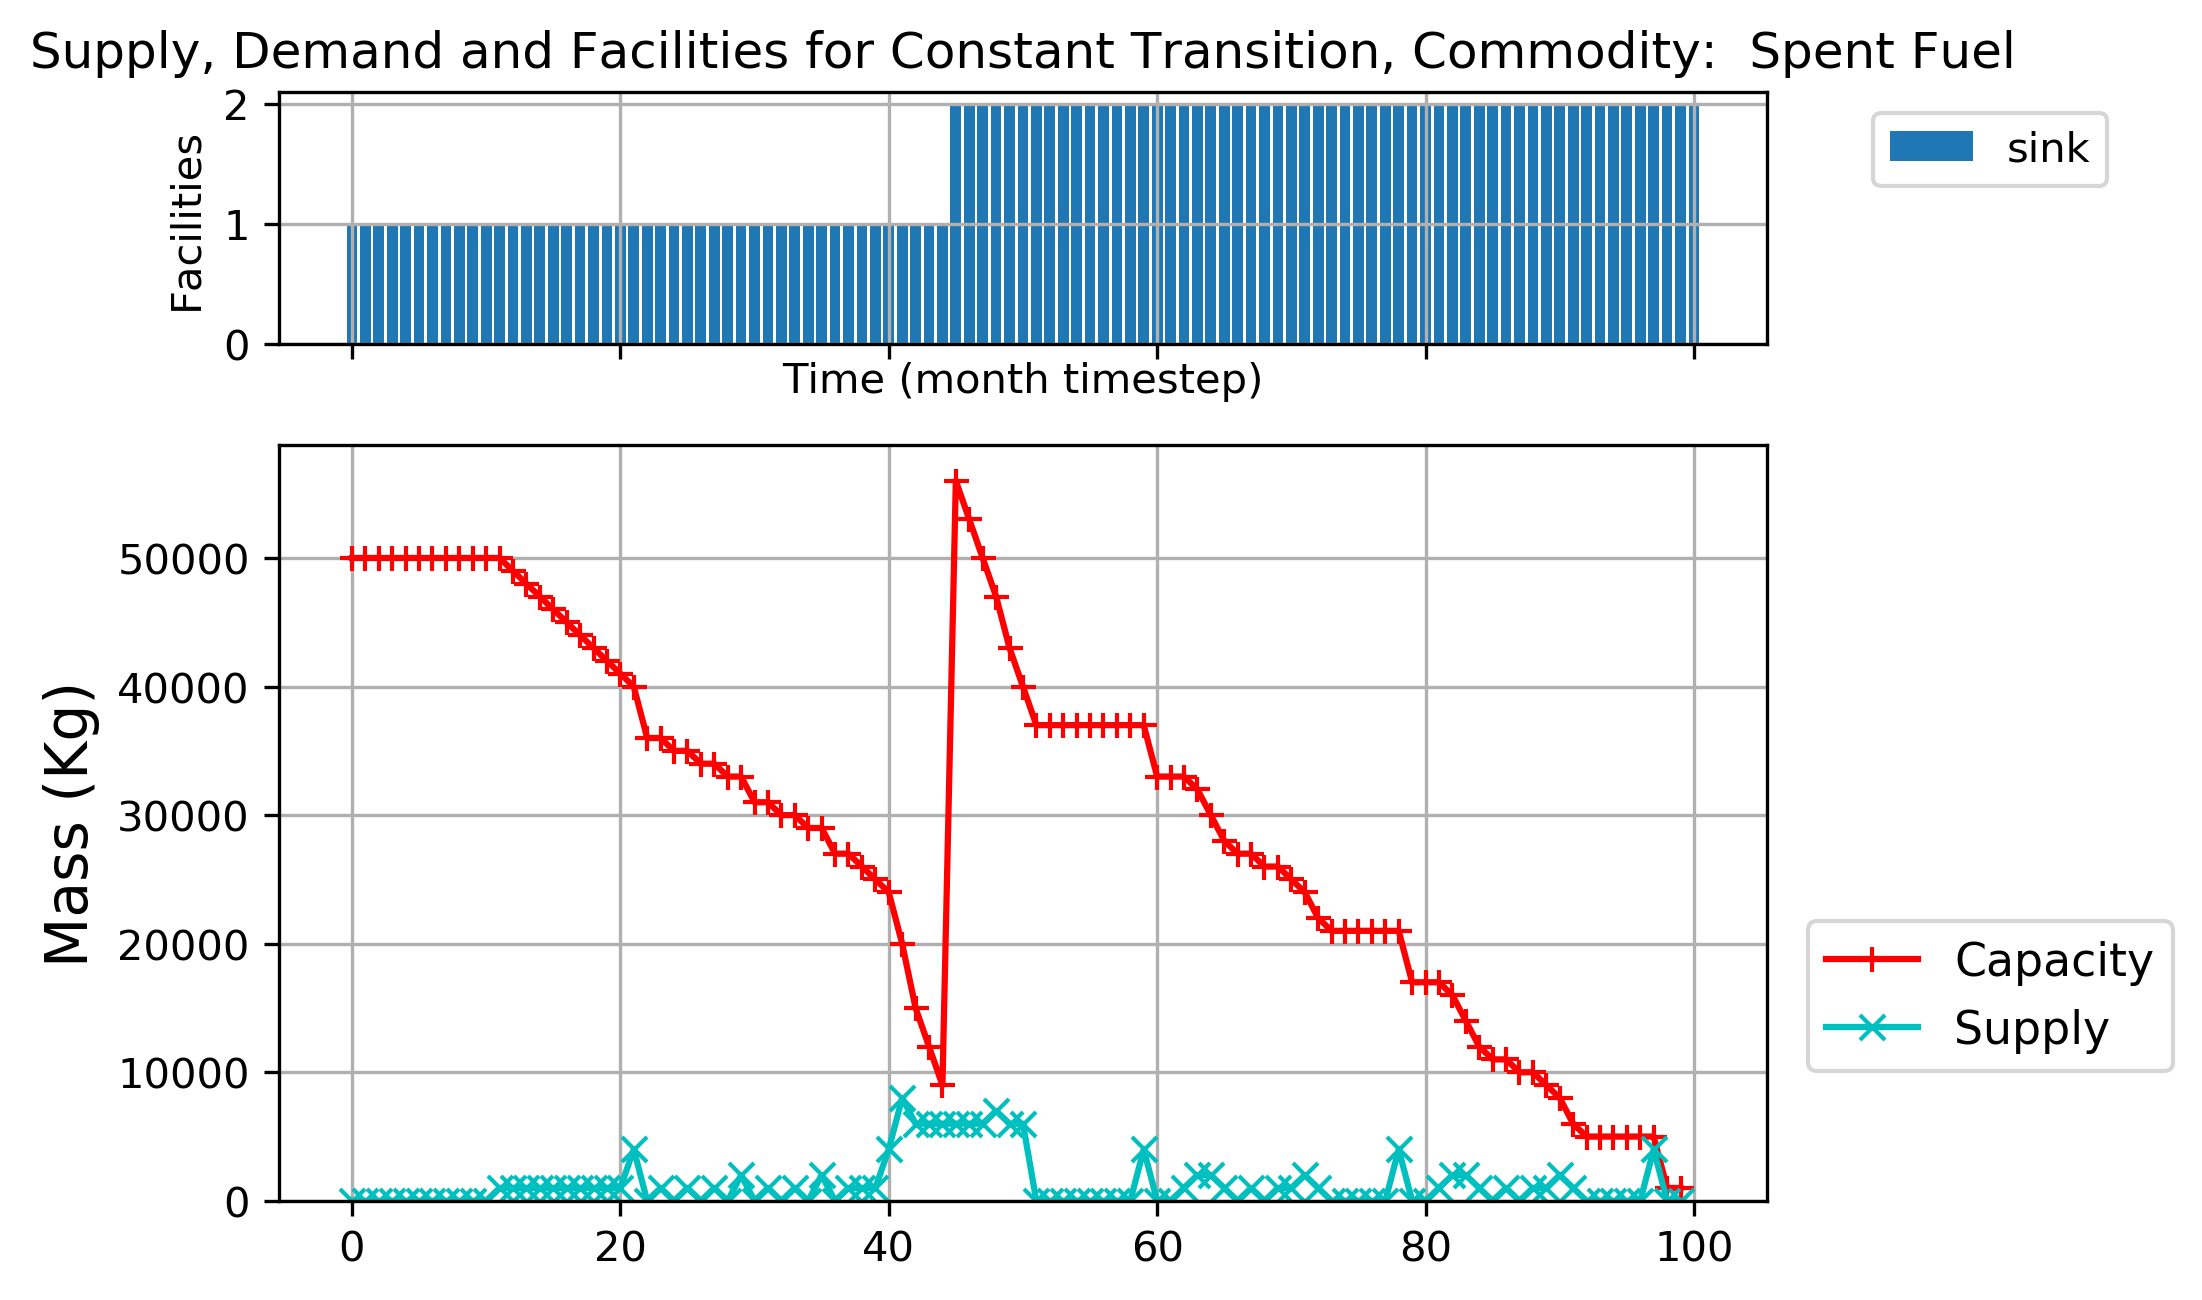
\includegraphics[width=\linewidth]{figures/constanttransition-spentfuel.png} 
            \caption{Spent Fuel is supplied by reactors and the capacity is provided by sink facilities.}
            \label{fig:constanttransition-spentfuel}
        \end{subfigure}
        \caption{Transition Scenario: Constant Power Demand of 10000MW}
    \end{figure}

    \subsubsection{\textbf{Basic Transition Scenario Simulation: Linearly Increasing Demand}}

    Figures \ref{fig:growingtransition-power}, \ref{fig:growingtransition-fuel}
    and \ref{fig:growingtransition-spentfuel} demonstrate the capability 
    of \deploy to deploy reactor and supporting facilities to meet the
    power demand and subsequently demanded secondary commodities 
    for a linearly increasing power demand. 
    A smaller supply buffer could be used while still minimizing under supply.
    Table \ref{tab:transition-scenario-results} shows the number of 
    undersupplied timesteps. 
    Figure \ref{fig:growingtransition-power} demonstrates that
    the main objective of \deploy (section \ref{sec:d3ploy}) 
    was met since there are no timesteps
    in which the supply of power falls under demand.
    
    \begin{figure}[]
        \centering
        \begin{subfigure}[t]{\textwidth}
        \centering
            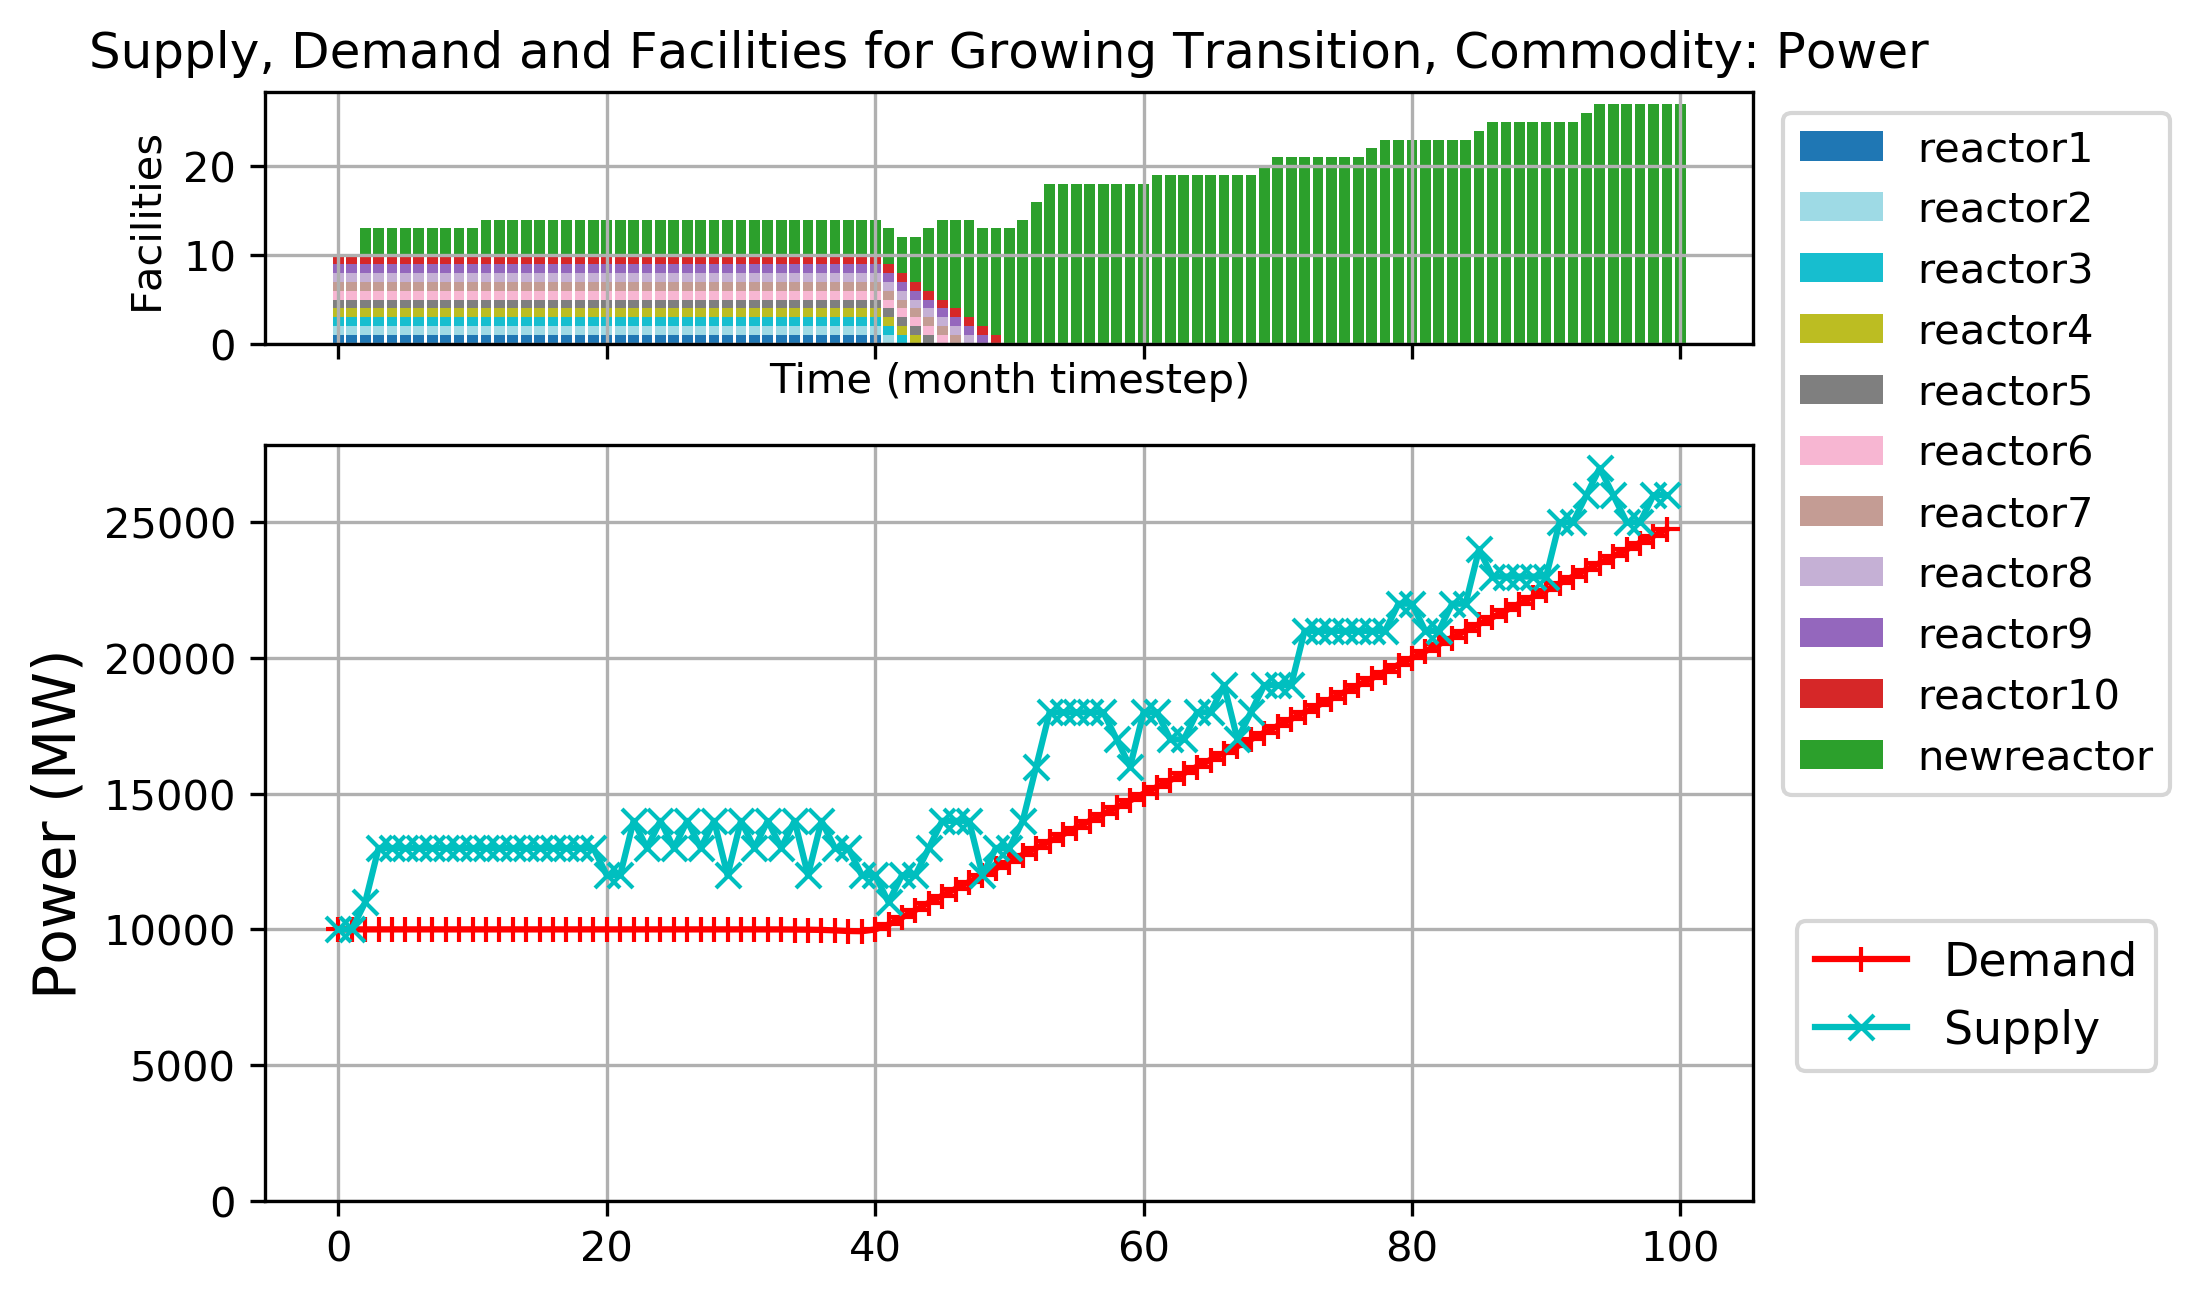
\includegraphics[width=0.7\linewidth]{figures/growingtransition-power.png} 
            \caption{The power demand is a user-defined equation and power is supplied by the reactors.}
            \label{fig:growingtransition-power}
        \end{subfigure}
        \begin{subfigure}[t]{0.6\textwidth}
            \centering
            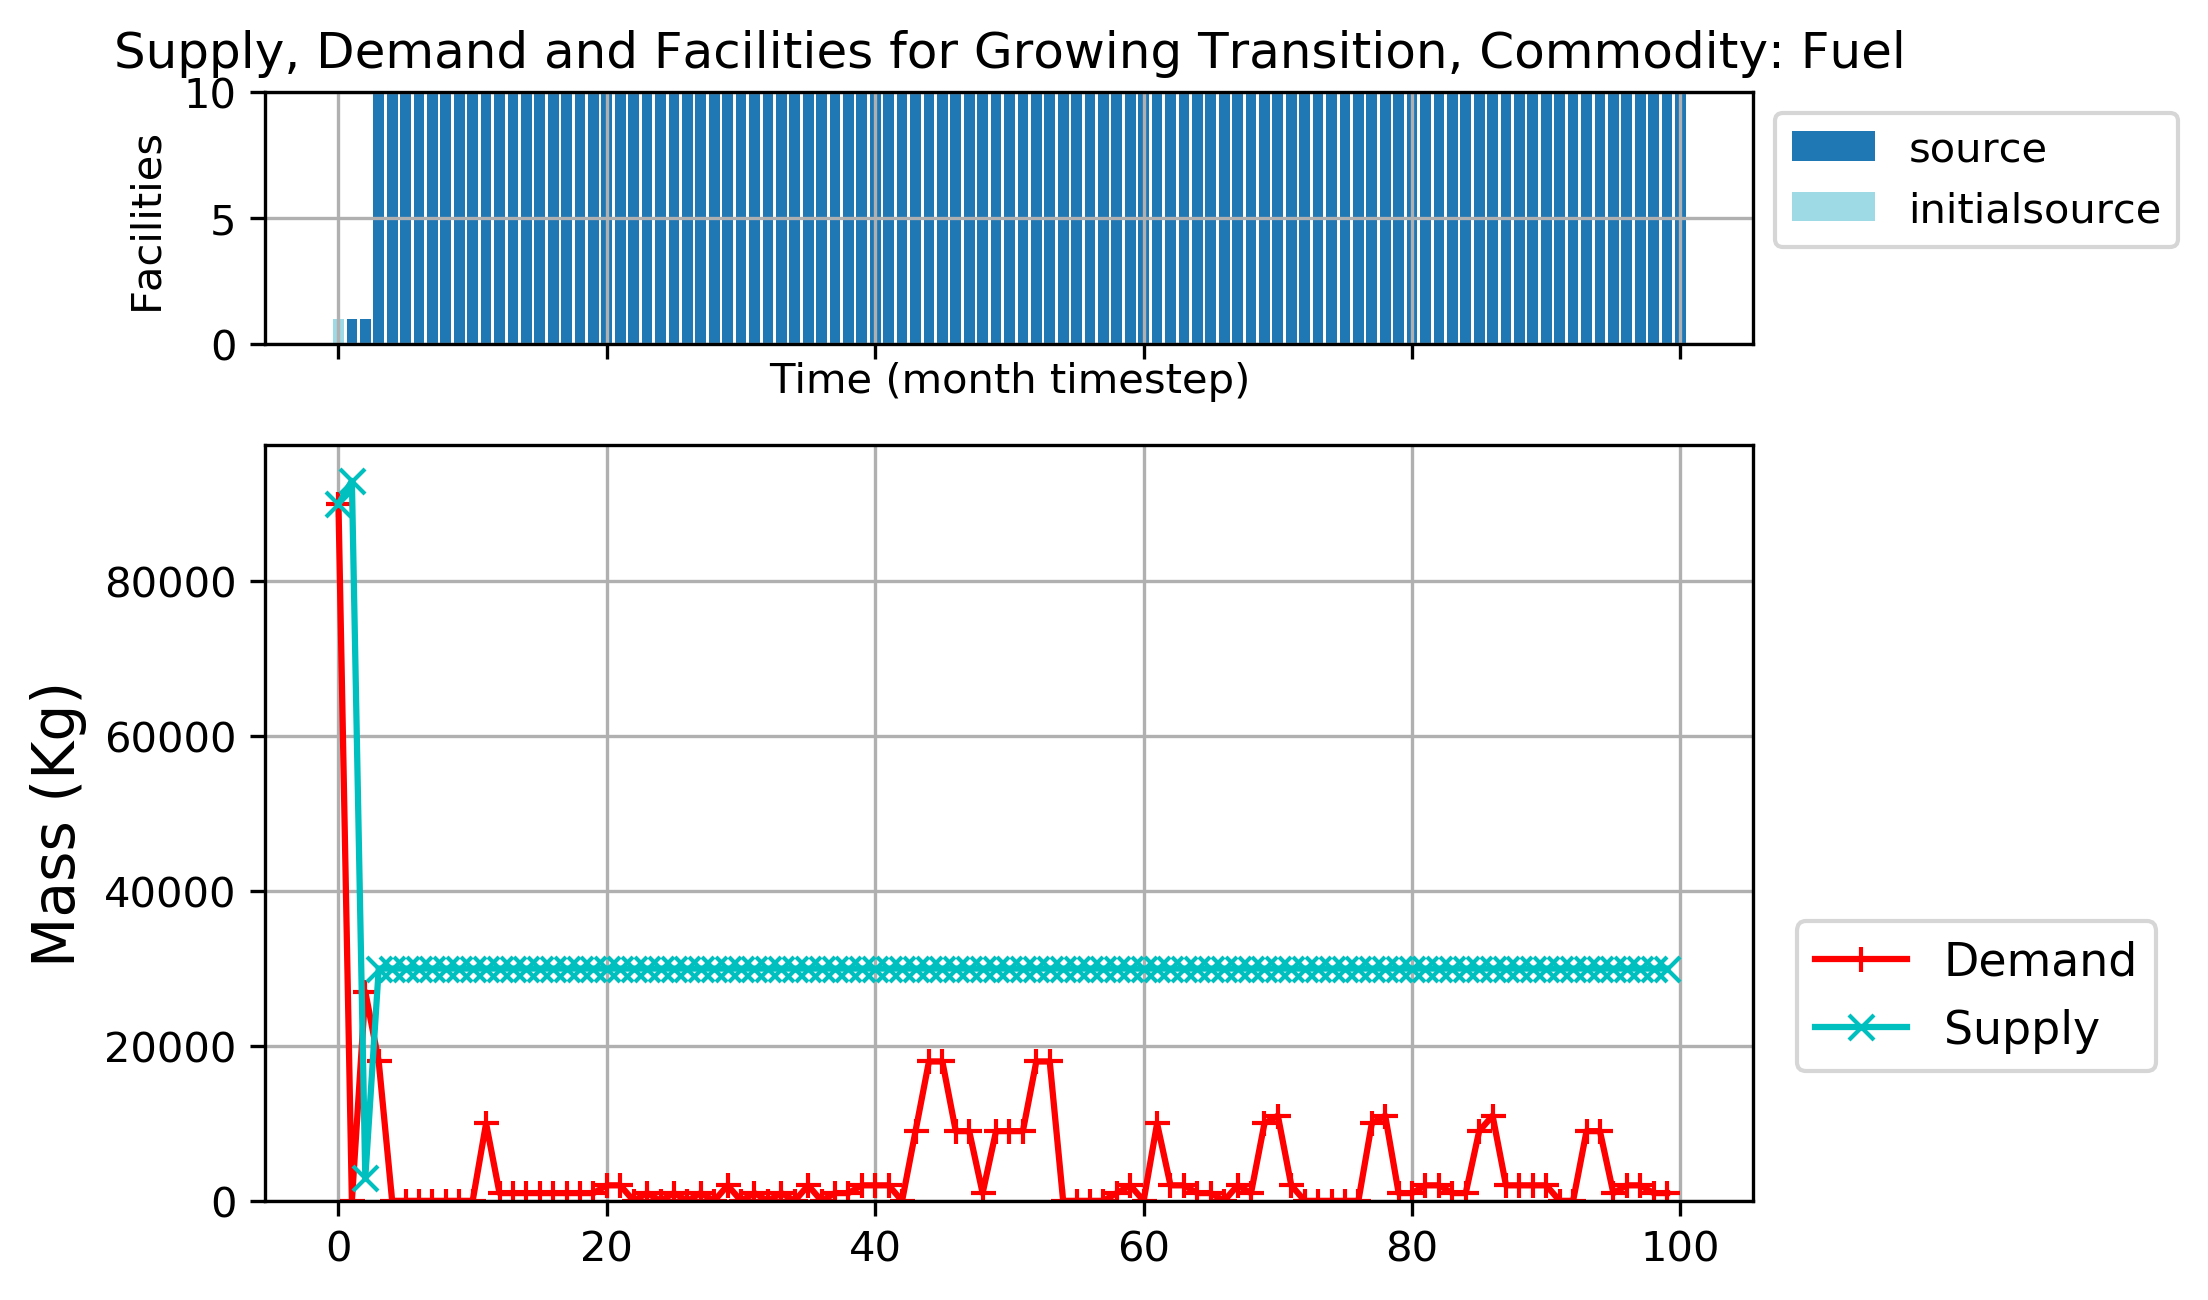
\includegraphics[width=\linewidth]{figures/growingtransition-fuel.png} 
            \caption{Fuel is demanded by reactors and supplied by source facilities.}
            \label{fig:growingtransition-fuel}
        \end{subfigure}
        \begin{subfigure}[t]{0.6\textwidth}
            \centering
            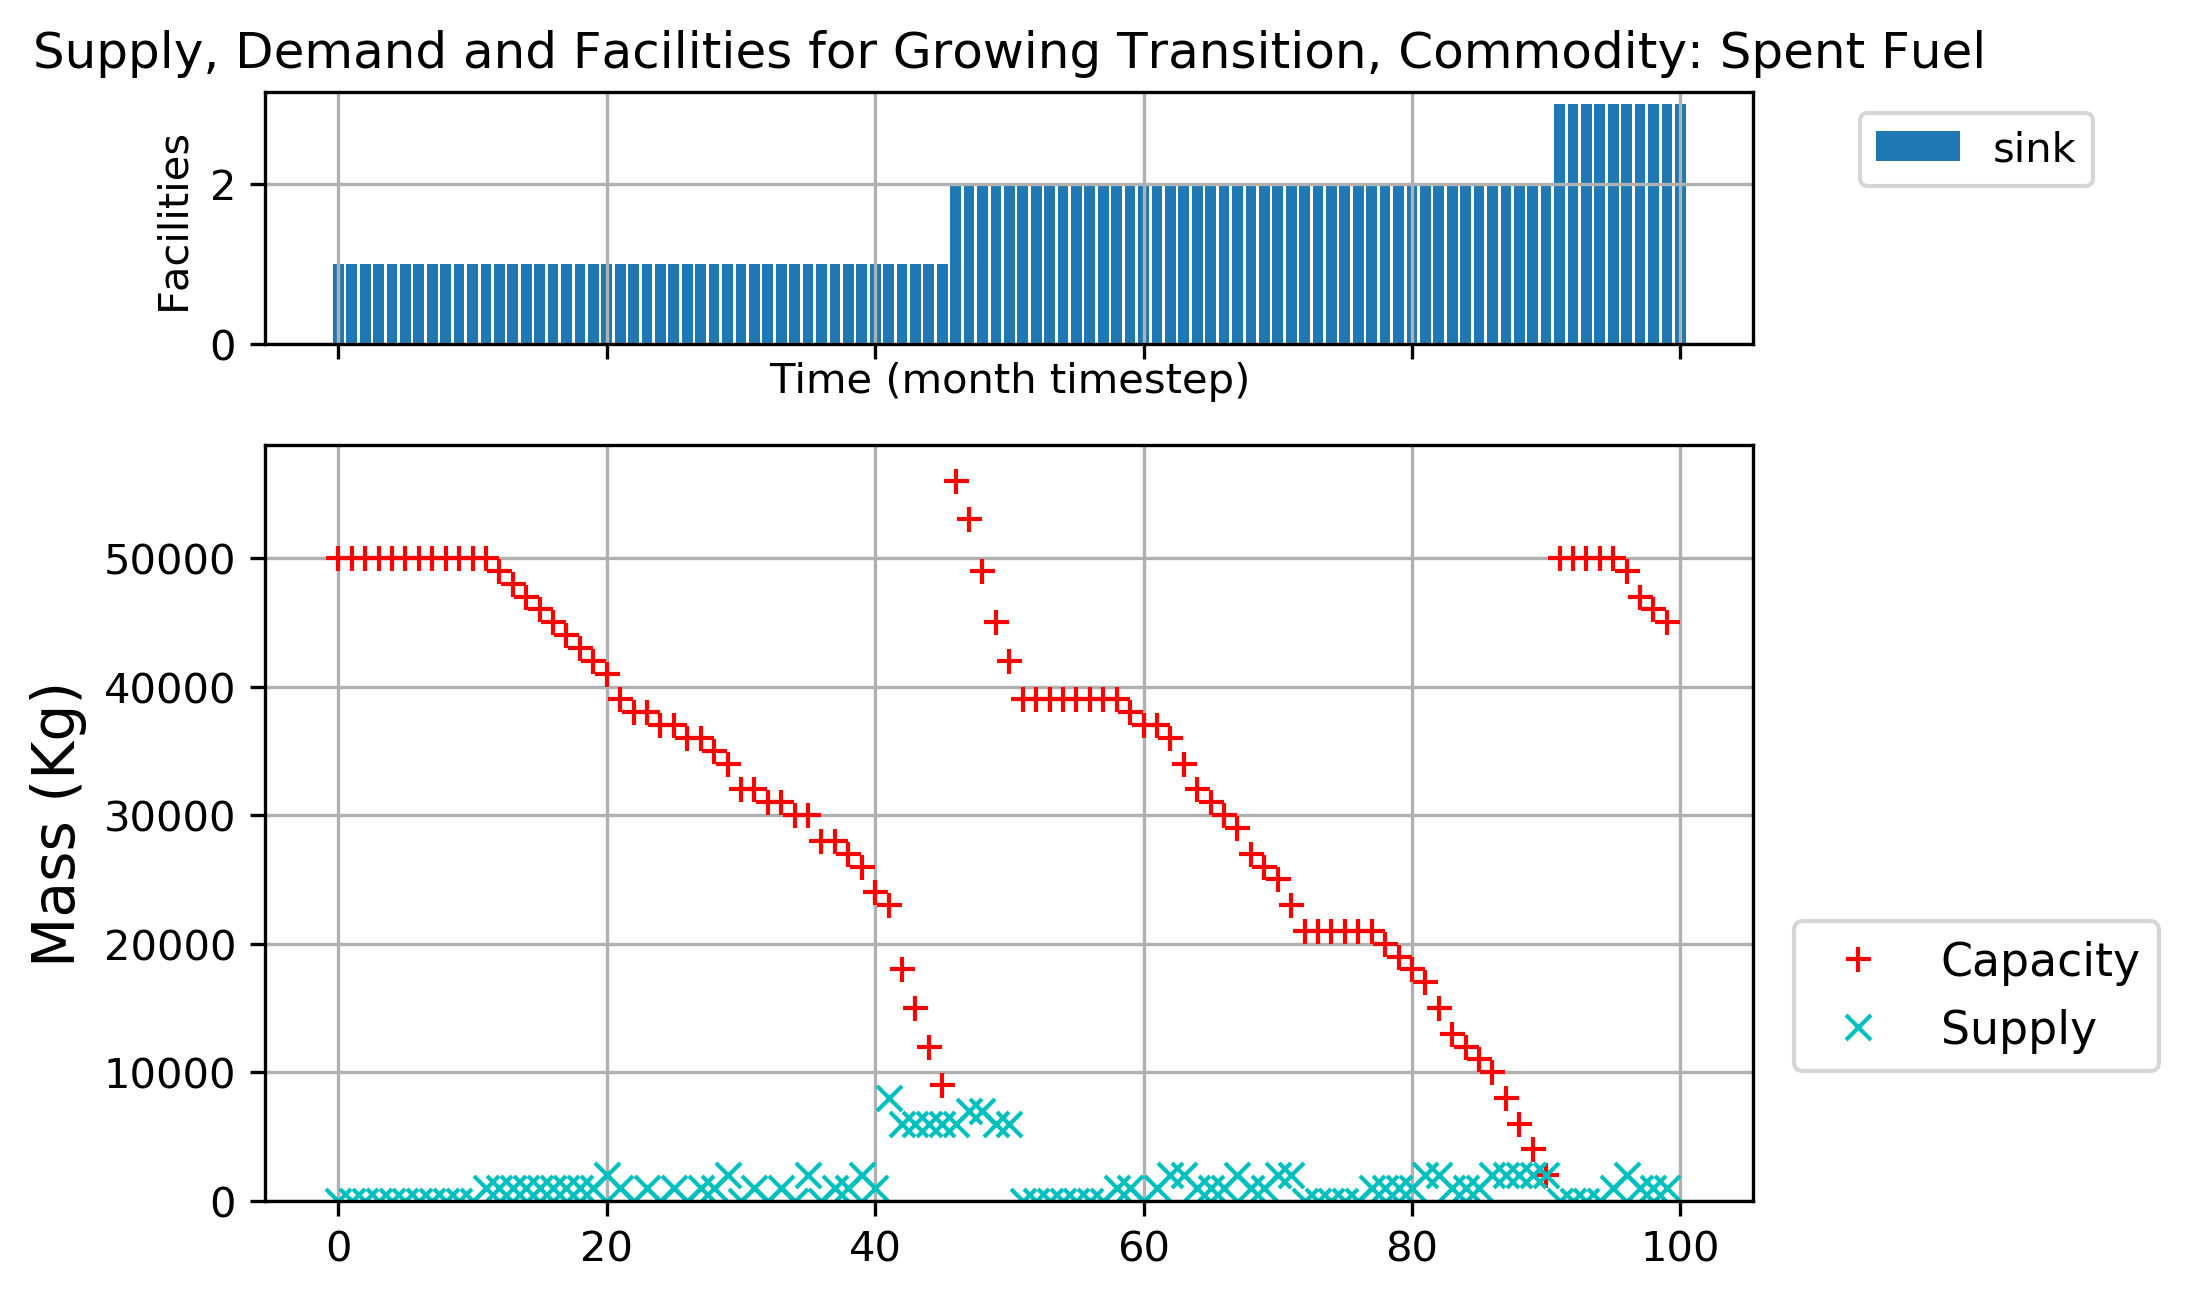
\includegraphics[width=\linewidth]{figures/growingtransition-spentfuel.png} 
            \caption{Spent Fuel is supplied by reactors and the capacity is provided by sink facilities.}
            \label{fig:growingtransition-spentfuel}
        \end{subfigure}
        \caption{Transition Scenario: Linearly increasing power demand.}
    \end{figure}
    
    \subsubsection{\textbf{Basic Transition Scenario Simulation: Sinusoidal Demand}}
    A sinusoidal power demand is the reflection of power demand in 
    the real world where power usage is higher in the winter and summer
    and lower in the spring and fall. 
    Figures \ref{fig:sinetransition-power}, \ref{fig:sinetransition-fuel}
    and \ref{fig:sinetransition-spentfuel} demonstrate the capability 
    of \deploy to deploy reactor and supporting facilities to meet the
    power demand and subsequently demanded secondary commodities 
    for a sinusoidal power demand. 
    Table \ref{tab:transition-scenario-results} shows the number of 
    undersupplied timesteps.
    
    For a sinusoidal power demand, the use of the triple exponential method
    for predicting demand is more effective than the 
    fast fourier transform method which was used for the constant 
    and linearly increasing power demand transition scenarios. 
    This is because the triple exponential smoothing method excels in
    forecasting data points for repetitive seasonal series of data. 
    
    \begin{figure}[]
        \centering
        \begin{subfigure}[t]{\textwidth}
        \centering
            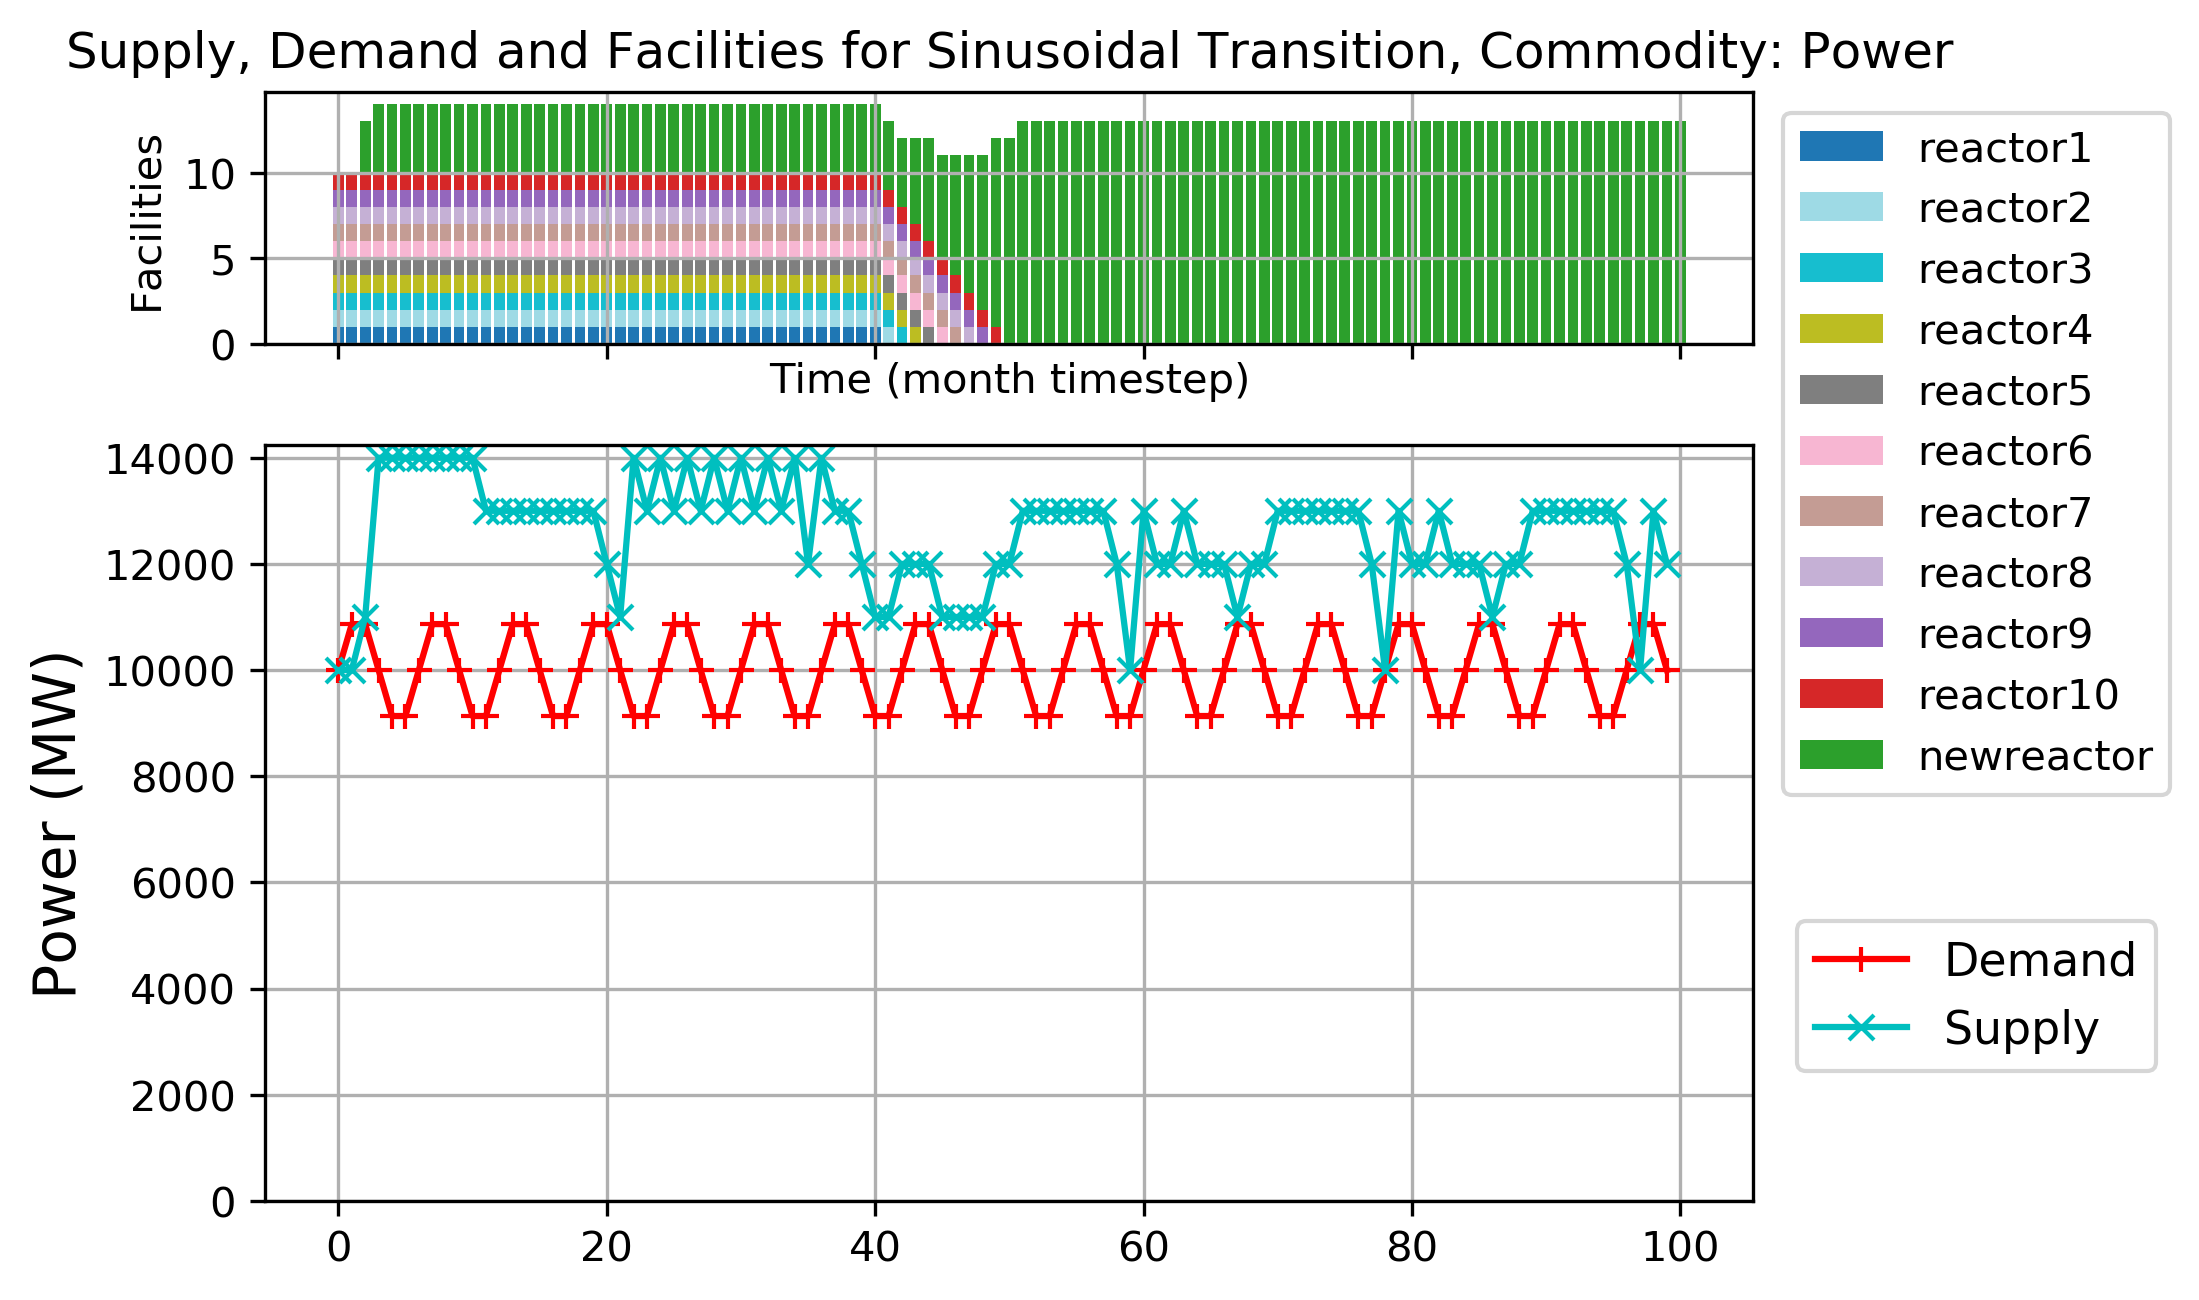
\includegraphics[width=0.7\linewidth]{figures/sinetransition-power.png} 
            \caption{The power demand is a user-defined equation and power is supplied by the reactors.}
            \label{fig:sinetransition-power}
        \end{subfigure}
        \begin{subfigure}[t]{0.6\textwidth}
            \centering
            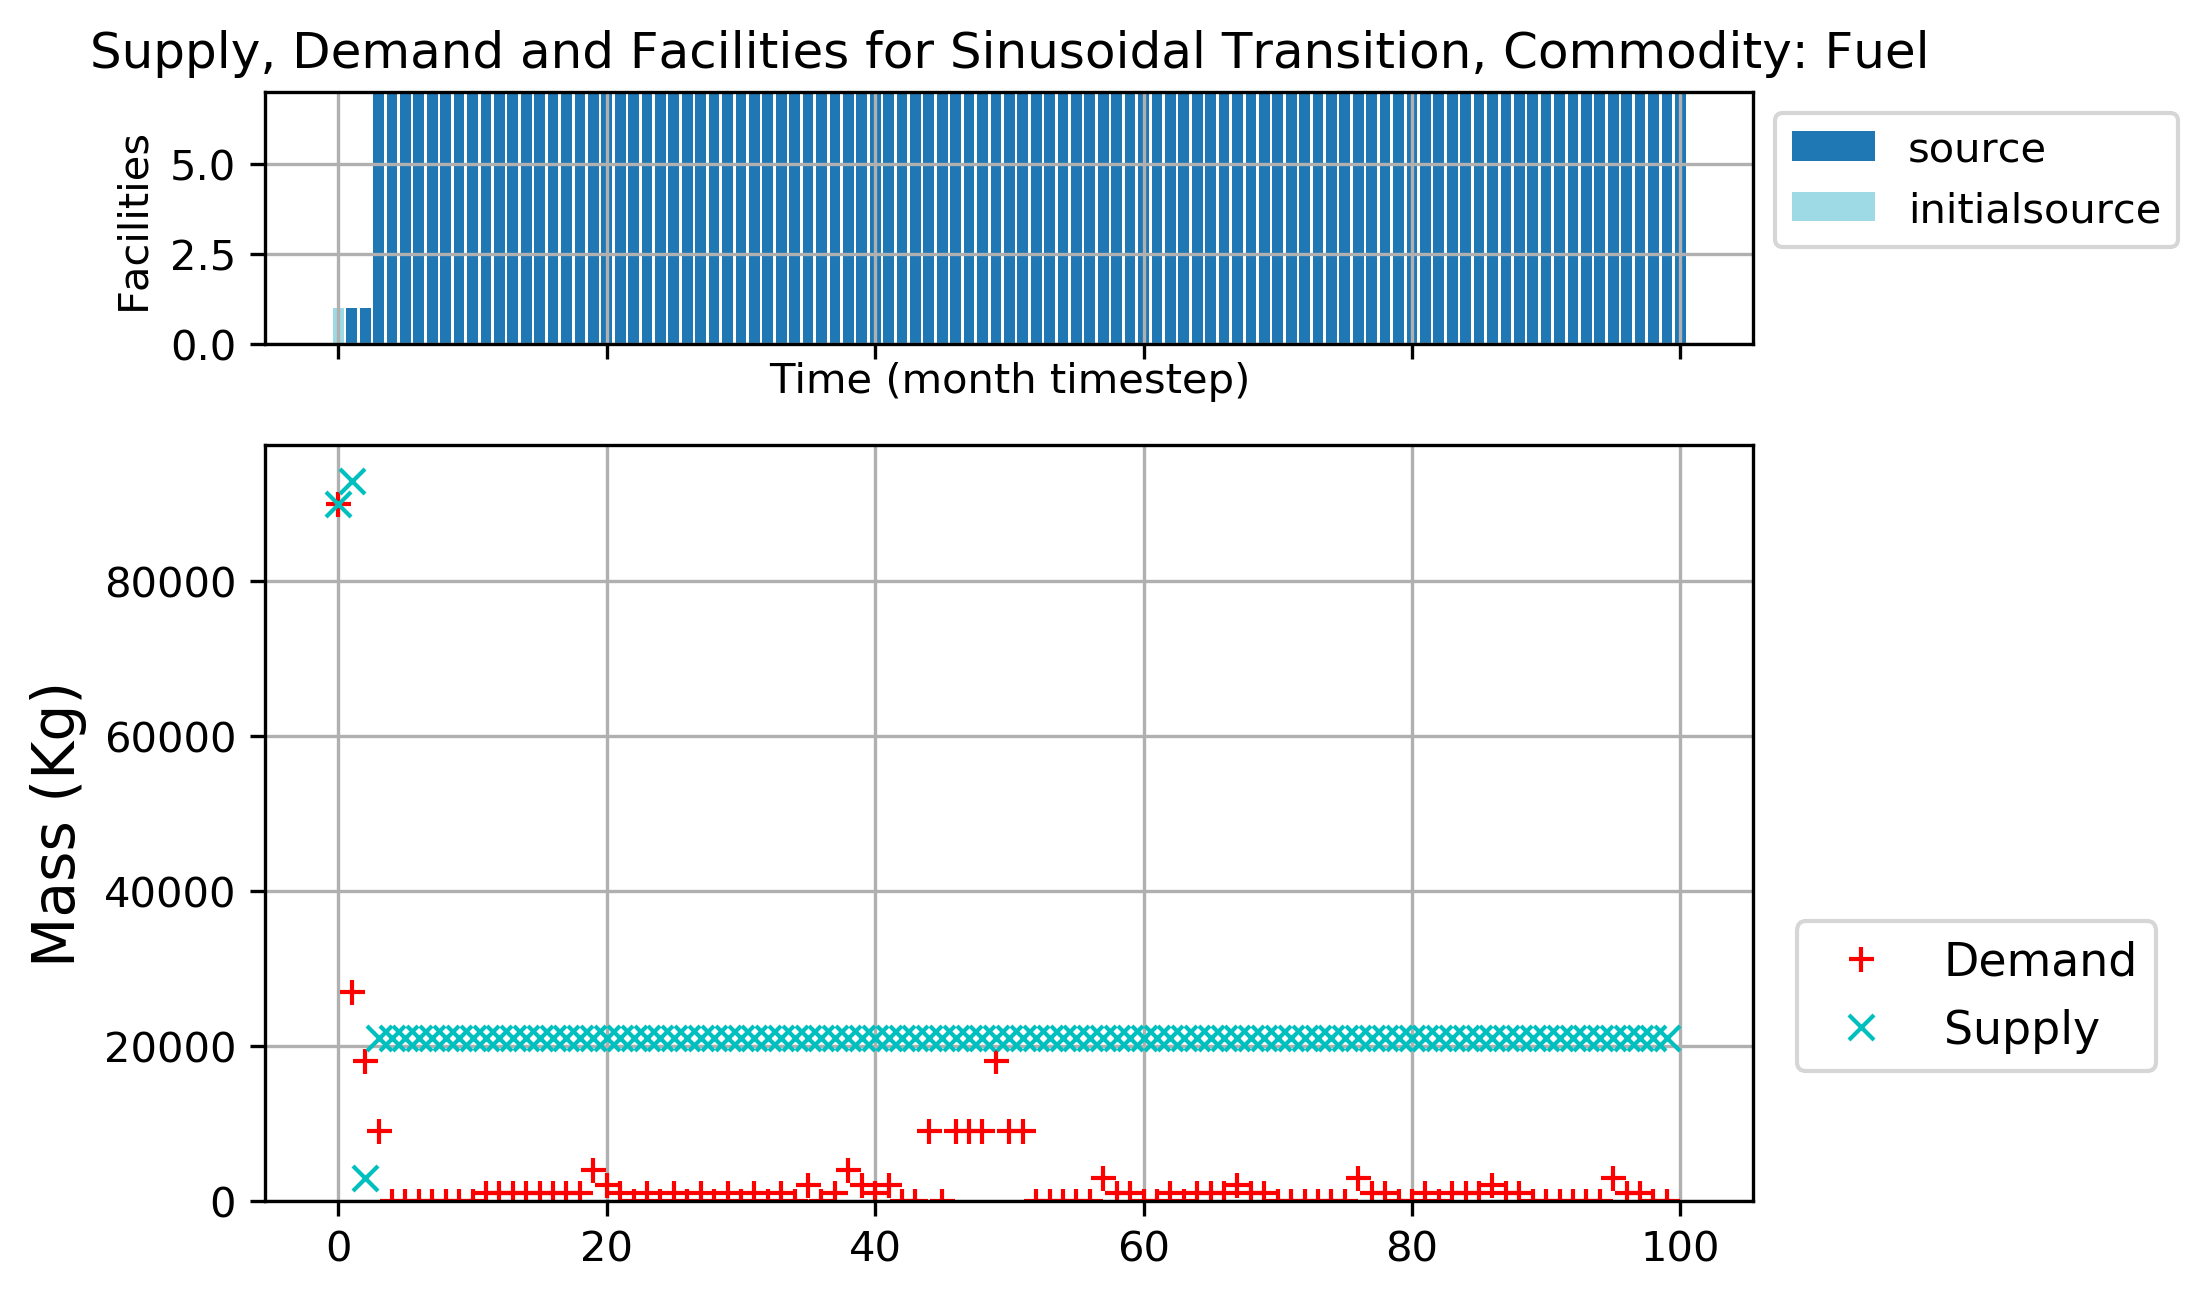
\includegraphics[width=\linewidth]{figures/sinetransition-fuel.png} 
            \caption{Fuel is demanded by reactors and supplied by source facilities.}
            \label{fig:sinetransition-fuel}
        \end{subfigure}
        \begin{subfigure}[t]{0.6\textwidth}
            \centering
            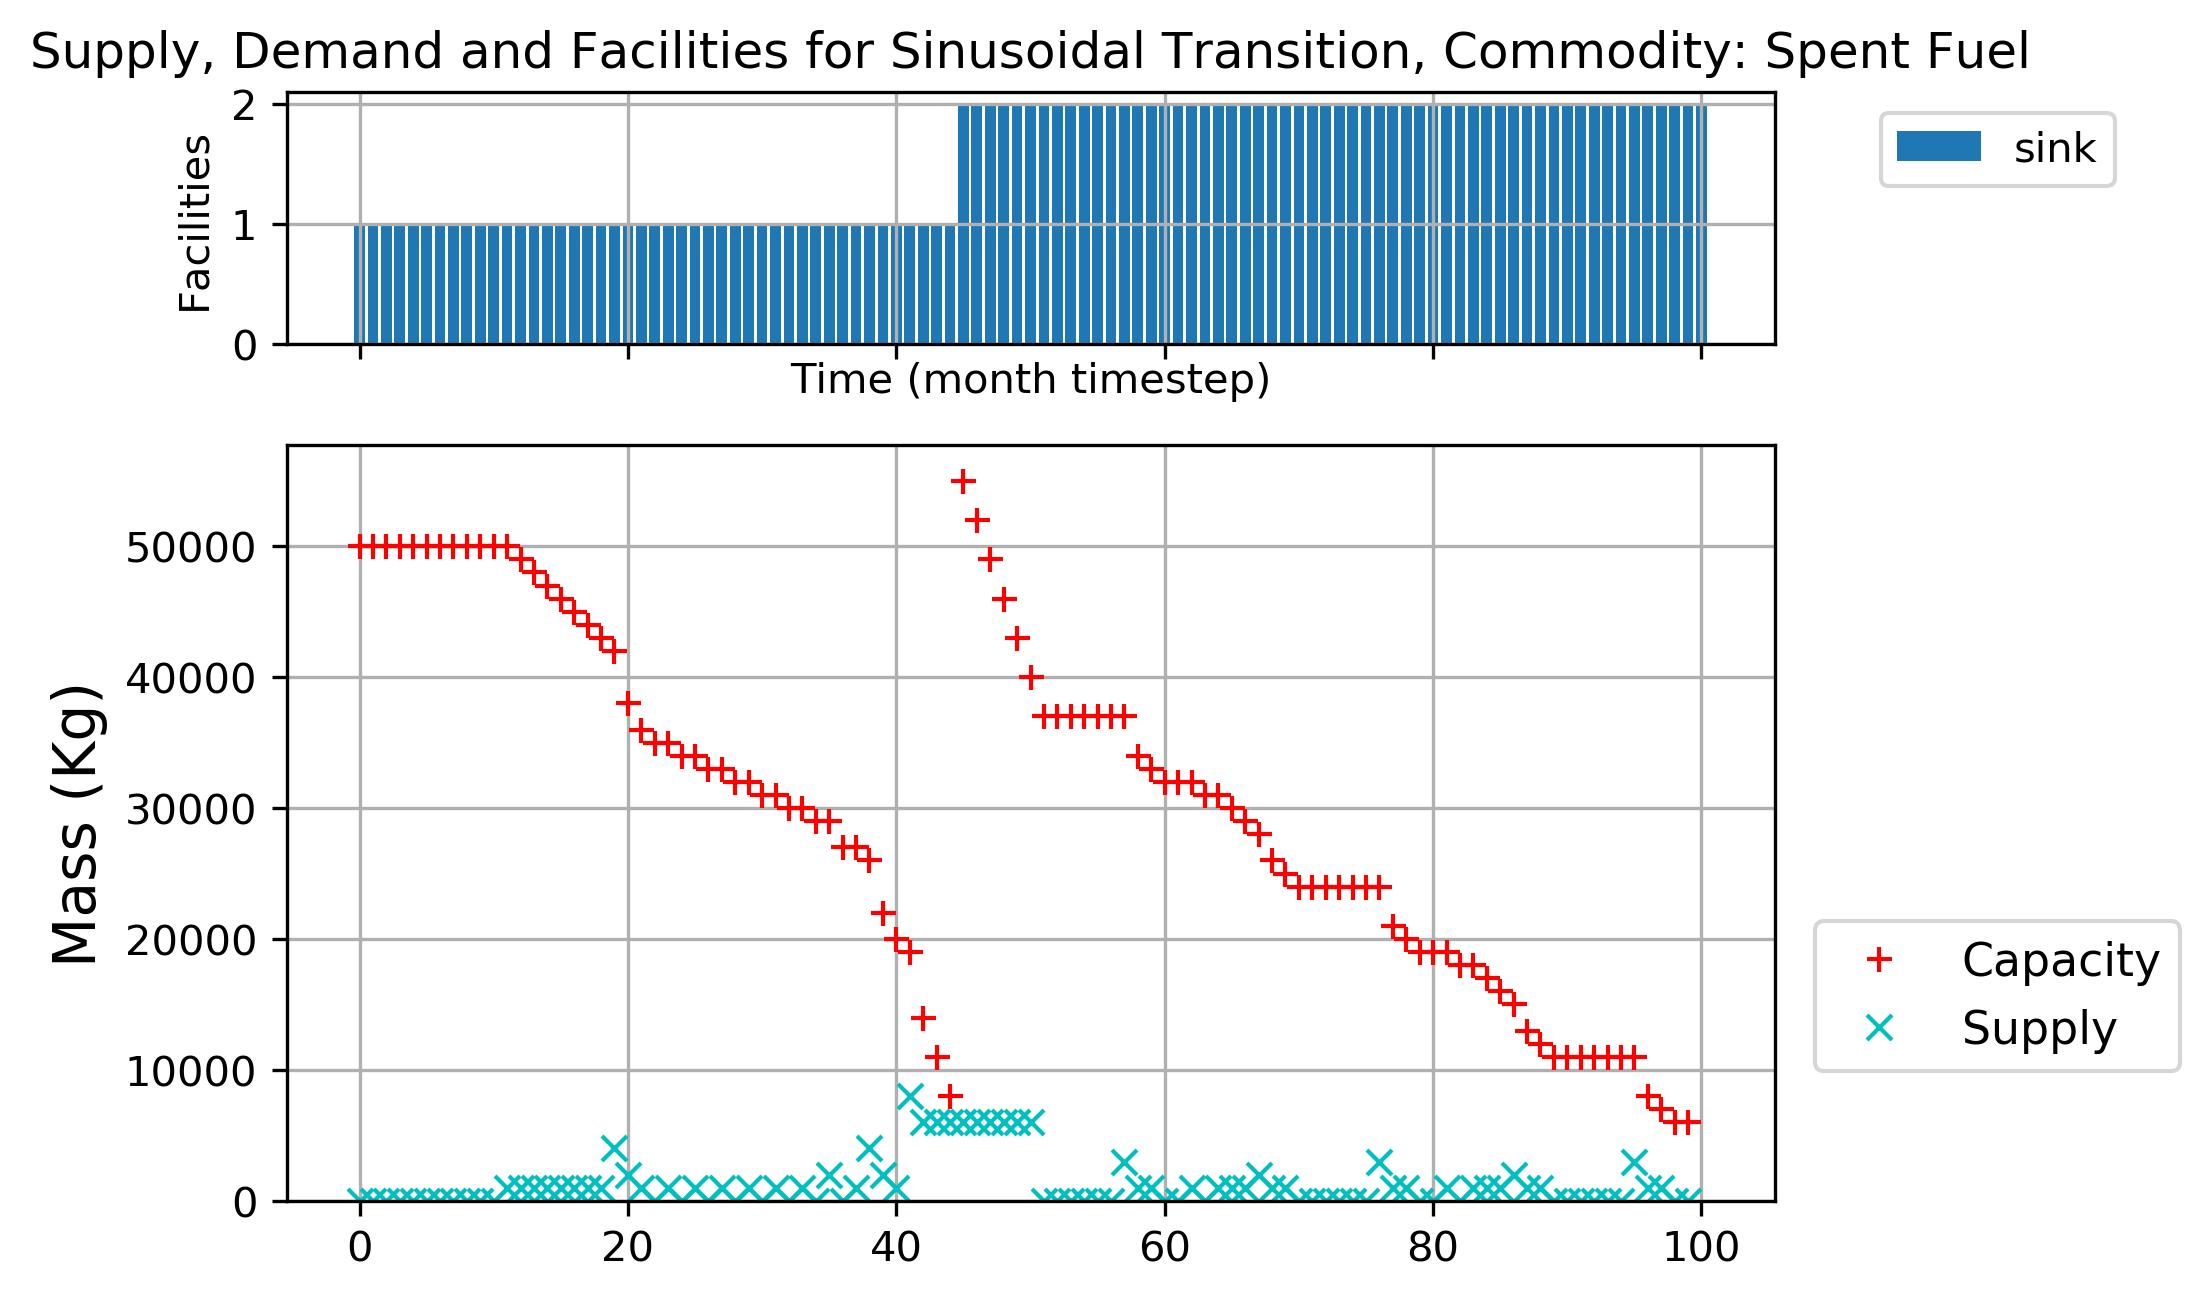
\includegraphics[width=\linewidth]{figures/sinetransition-spentfuel.png} 
            \caption{Spent Fuel is supplied by reactors and the capacity is provided by sink facilities.}
            \label{fig:sinetransition-spentfuel}
        \end{subfigure}
        \caption{Transition Scenario: Sinusoidal Power Demand}
    \end{figure}
    
    \begin{table}[]
        \centering
        \caption {Undersupply results for each commodity in each scenario}
        \label{tab:transition-scenario-results}
        \begin{tabular}{|l|l|p{4cm}|}
        \hline
        \textbf{Basic Transition Scenario}    & \textbf{Commodity}    & \textbf{No. of timesteps with undersupply} \\ \hline
        \multirow{2}{*}{\textbf{Constant Power}} & Fuel & 1 \\ \cline{2-3}
                                                 & Power & 0 \\ \cline{2-3}
                                                 & Spent Fuel & 0 \\ \hline
        \multirow{2}{*}{\textbf{Linearly Increasing Power}} & Fuel & 1 \\ \cline{2-3}
                                                 & Power & 0 \\ \cline{2-3}
                                                 & Spent Fuel & 0 \\ \hline
        \multirow{2}{*}{\textbf{Sinusoidal Power}} & Fuel & 1 \\ \cline{2-3}
                                                 & Power & 1 \\ \cline{2-3}
                                                 & Spent Fuel & 0 \\ \hline
        \end{tabular}
    \end{table}

\section{DYMOND}
DYMOND \cite{yacout_modeling_2005} is a \gls{NFCSim} run within 
the AnyLogic software with Microsoft Excel templates for 
data input and output. 
The major inputs to this code are reactor and fuel cycle 
characteristics, and time-dependent power demand 
\cite{feng_standardized_2016}.   
The code calls ORIGEN \cite{bell_origen_1973} during the simulation 
to conduct reactor depletion calculations. 
The mass flows and inventories are recorded at a system-level
and individual isotopes are tracked. 
DYMOND's main design objective is ease of understanding it's 
behavior and variables. 

In DYMOND, reactor facilities are automatically deployed to 
meet a user-defined power demand and the user can define 
the targeted shares of energy for up to five reactor types. 
The user also defines the fuel loading model used to calculate 
reactor spent fuel compositions, the type of reprocessing 
technology that is used for each reactor type, and the length 
of used fuel cooling time etc. 
In DYMOND, the user must define the deployment schedule for 
the reprocessing plants and the cooling pools and storage pools 
are all assumed to have infinite capacities. 
DYMOND does not have demand-driven deployment capabilities for 
supporting fuel cycle facilities. 

The difference between \Cyclus and DYMOND is that \Cyclus uses 
agent-based modeling for all facilities and mass flows, 
whereas DYMOND uses fleet-based modeling for all facilities and 
mass flows with exception of reactor facilities. 
\Cyclus has the advantage of flexibility and customization, 
and DYMOND has the advantage of ease of use. 

\section{Sensitivity Analysis Capabilities}
In this work, \Cyclus and DYMOND were coupled with Dakota 
\cite{eldred_dakota_2010} to give the \glspl{NFCSim} \gls{SA}, 
\gls{UQ}, and optimization capabilities. 